
\documentclass{beamer}
\usetheme{ucl}

\usepackage[utf8]{inputenc}


%%% Increase the height of the banner: the argument is a scale factor >=1.0
%\setbeamertemplate{banner}[ucl][10.0]

%%% Change the colour of the main banner
%%% The background should be one of the UCL colours (except pink or white):
%%%   black,darkpurple,darkred,darkblue,darkgreen,darkbrown,richred,midred,
%%%   navyblue,midgreen,darkgrey,orange,brightblue,brightgreen,lightgrey,
%%%   lightpurple,yellow,lightblue,lightgreen,stone
\setbeamercolor{banner}{bg=darkpurple}
%\setbeamercolor{banner}{bg=yellow,fg=black}

%%% Add a stripe behind the banner
%\setbeamercolor{banner stripe}{bg=darkpurple,fg=black}

%%% The main structural elements
\setbeamercolor{structure}{fg=black}

%%% Author/Title/Date and slide number in the footline
\setbeamertemplate{footline}[author title date]

%%% Puts the section/subsection in the headline
% \setbeamertemplate{headline}[section]

%%% Puts a navigation bar on top of the banner
%%% For this to work correctly, the each \section command needs to be
%%% followed by a \subsection. Requires one extra compile.
% \setbeamertemplate{headline}[miniframes]
%%% Accepts an optional argument determining the width
% \setbeamertemplate{headline}[miniframes][0.3\paperwidth]


%%% Puts the frame title in the banner
%%% Won't work correctly with the above headline templates
%\useoutertheme{ucltitlebanner}
%%% Similar to above, but smaller (and puts subtitle on same line as title)
\useoutertheme[small]{ucltitlebanner}

%%% Gives block elements (theorems, examples) a border
% \useinnertheme{blockborder}
%%% Sets the body of block elements to be clear
% \setbeamercolor{block body}{bg=white,fg=black}

%%% Include CSML logo on title slide
%\titlegraphic{\includegraphics[width=0.16\paperwidth]{csml_logo}}

%%% Include CSML logo in bottom right corner of all slides
%\logo{\includegraphics[width=0.12\paperwidth]{csml_logo}}

%%% Set a background colour
% \setbeamercolor{background canvas}{bg=lightgrey}

%%% Set a background image
%%% Some sample images are available from the UCL image store:
%%%   https://www.imagestore.ucl.ac.uk/home/start
% \setbeamertemplate{background canvas}{%
%   \includegraphics[width=\paperwidth]{imagename}}



%%%%%% Some other settings that can make things look nicer
%%% Set a smaller indent for description environment
\setbeamersize{description width=2em}
%%% Remove nav symbols (and shift any logo down to corner)
\setbeamertemplate{navigation symbols}{\vspace{-2ex}}








\DeclareMathOperator{\Cov}{Cov}
\DeclareMathOperator{\Var}{Var}
\DeclareMathOperator{\E}{\mathbb{E}}
\DeclareMathOperator{\Proba}{\mathbb{P}}

\newcommand{\Covb}[2]{\ensuremath{\Cov\!\left[#1,#2\right]}}
\newcommand{\Eb}[1]{\ensuremath{\E\!\left[#1\right]}}
\newcommand{\Pb}[1]{\ensuremath{\Proba\!\left[#1\right]}}
\newcommand{\Varb}[1]{\ensuremath{\Var\!\left[#1\right]}}

% norm
\newcommand{\norm}[1]{\| #1 \|}

\newcommand{\indep}{\rotatebox[origin=c]{90}{$\models$}}





\usepackage{mathptmx,amsmath,amssymb,graphicx,bibentry,bbm,ragged2e}
\usepackage[english]{babel}

\makeatletter

\newcommand{\noun}[1]{\textsc{#1}}
\newcommand{\jitem}[1]{\item \begin{justify} #1 \end{justify} \vfill{}}
\newcommand{\sframe}[2]{\frame{\frametitle{#1} #2}}

\newenvironment{centercolumns}{\begin{columns}[c]}{\end{columns}}
%\newenvironment{jitem}{\begin{justify}\begin{itemize}}{\end{itemize}\end{justify}}



%\usetheme{Warsaw}
%\setbeamertemplate{footline}[text line]{}
%\setbeamertemplate{headline}{}
%\setbeamercolor{structure}{fg=purple!50!blue, bg=purple!50!blue}

%\setbeamersize{text margin left=15pt,text margin right=15pt}

%\setbeamercovered{transparent}


\@ifundefined{showcaptionsetup}{}{%
 \PassOptionsToPackage{caption=false}{subfig}}
\usepackage{subfig}

\usepackage[utf8]{inputenc}
\usepackage[T1]{fontenc}

\usepackage{multirow}


\makeatother

\def \draft {1}

\usepackage{xparse}
\usepackage{ifthen}
\DeclareDocumentCommand{\comment}{m o o o o}
{\ifthenelse{\draft=1}{
    \textcolor{red}{\textbf{C : }#1}
    \IfValueT{#2}{\textcolor{blue}{\textbf{A1 : }#2}}
    \IfValueT{#3}{\textcolor{ForestGreen}{\textbf{A2 : }#3}}
    \IfValueT{#4}{\textcolor{red!50!blue}{\textbf{A3 : }#4}}
    \IfValueT{#5}{\textcolor{Aquamarine}{\textbf{A4 : }#5}}
 }{}
}
\newcommand{\todo}[1]{
\ifthenelse{\draft=1}{\textcolor{red!50!blue}{\textbf{TODO : \textit{#1}}}}{}
}




\begin{document}

\title
[Open transportation models]{Estimating public transport congestion in UK urban areas with open transport models}
\author[Raimbault]{J.~Raimbault$^{1,2,3,\ast}$ and M.~Batty$^{1}$\\\medskip
$^{\ast}$\texttt{j.raimbault@ucl.ac.uk}
}

\institute[UCL]{$^{1}$Center for Advanced Spatial Analysis, University College London\\
$^{2}$UPS CNRS 3611 Complex Systems Institute Paris\\
$^{3}$UMR CNRS 8504 G{\'e}ographie-cit{\'e}s
}




\date[14/04/2021]{GISRUK 2021\\
Session Transport I: Analysis and Modelling\\
April 14th, 2021\\
}

\frame{\maketitle}

  % Operational urban transport models require to gather heterogeneous sets of data and often integrate different sub-models. Their systematic validation and reproducible application therefore remains problematic. We propose in this contribution to build transport models from the bottom-up using scientific workflow systems with open-source components and data. These open models are aimed in particular at estimating congestion of public transport in all UK urban areas. This allows us building health indicators related to public transport density in the context of the COVID-19 crisis, and testing related policies.


\section{Introduction}


\sframe{}{

% With the COVID-19 crisis and associated social distancing requirements, public transport has been designed and perceived as a risky environment (Tirachini and Cats, 2020), besides loosing ridership due to drops in mobility and modal shift (Gutiérrez et al., 2020). A detailed understanding of how work and transport related policies impacts effective densities in public transport is therefore an important issue. When systematically designing and testing transport policies, a reproducible and validated workflow is crucial first to ensure comparability between different case studies, but also to be able to apply them on a large set of urban areas.



}



\sframe{Urban transportation models}{

% Urban transportation models such as four-step models, and more generally land-use transport interaction models (Wegener, 2004), require the integration of heterogenous data and the coupling of various submodules with possibly high levels of complexity. 


\textit{MATSim model: heterogenous data and integration of many sub-models}

\medskip

\begin{center}
	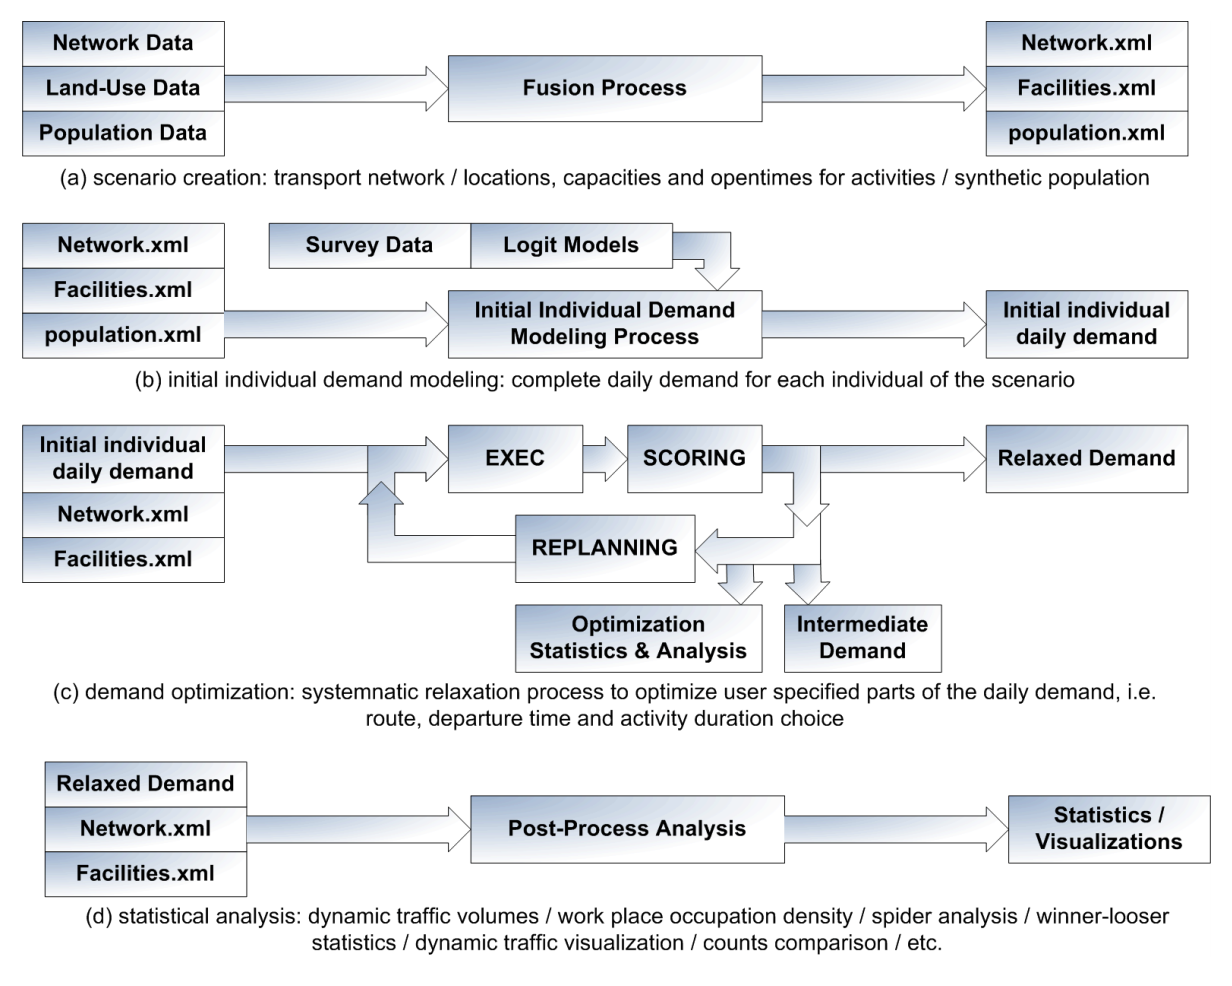
\includegraphics[height=0.7\textheight]{figures/matsim.png}	
\end{center}

Source: \cite{balmer2009matsim}

}

\sframe{Land-use transport models}{

\textit{Land-use transport models as a progressive complexification through coupling of detailed sub-models}

\medskip

\begin{center}
	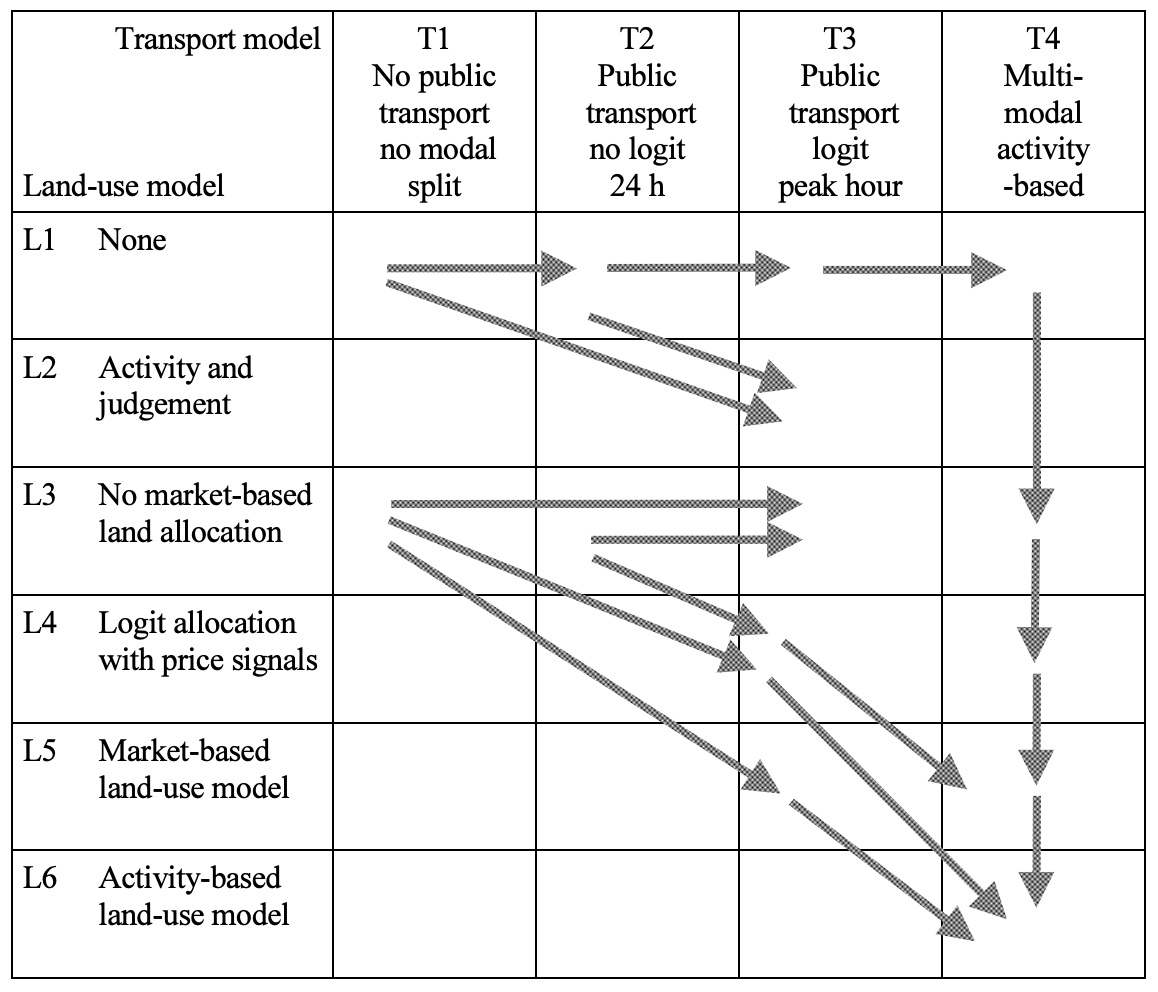
\includegraphics[width=0.45\linewidth]{figures/wegener1.png}\hspace{0.3cm}
	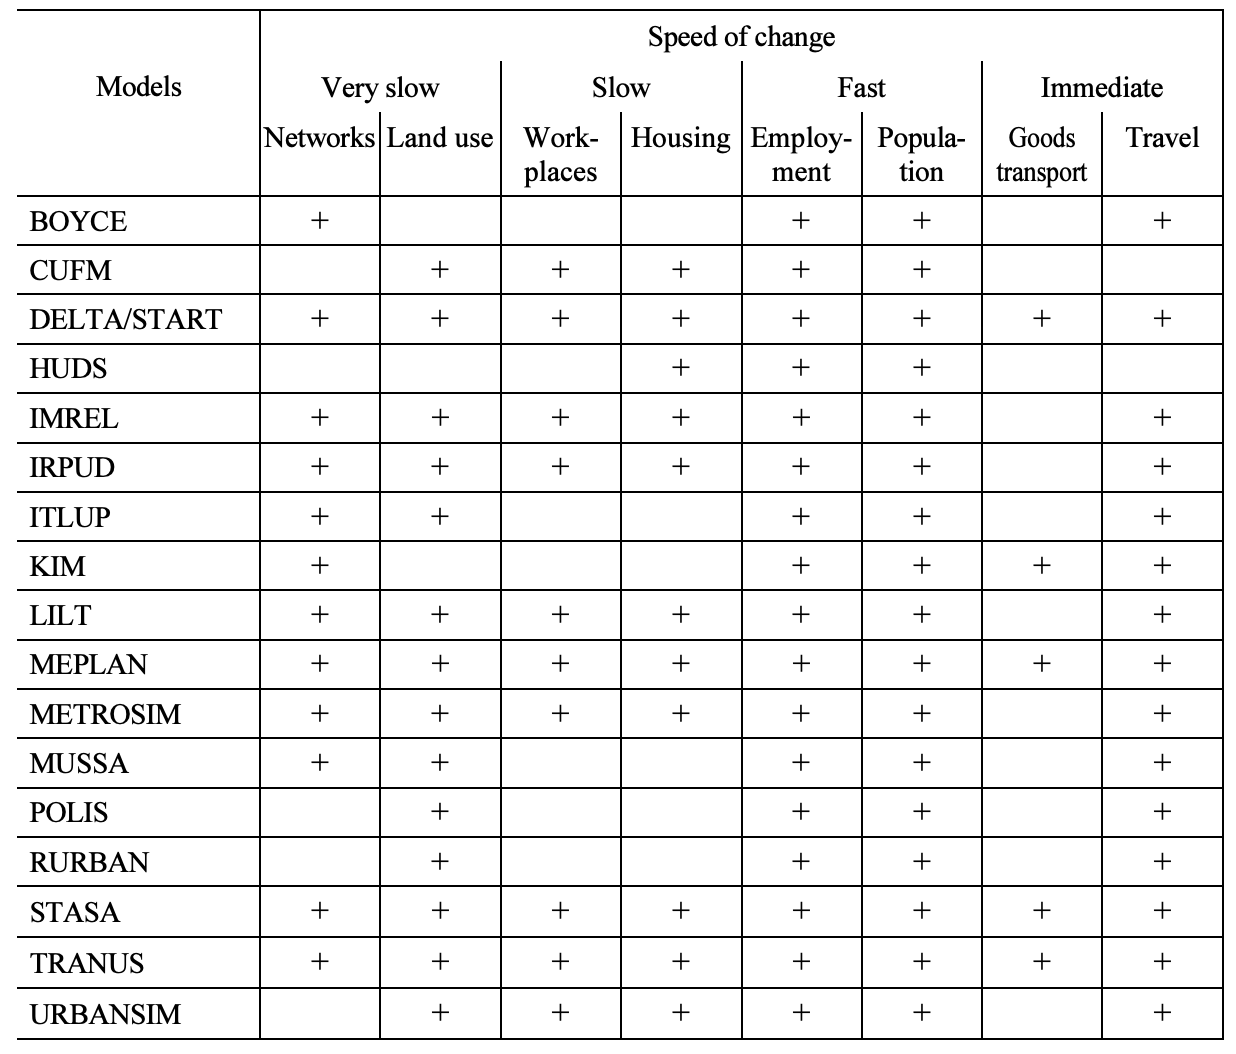
\includegraphics[width=0.45\linewidth]{figures/wegener2.png}
\end{center}

Source: \cite{wegener2004land}

}

\sframe{Relevance of large scale models}{

%This raises issues on the one hand for their implementation, transferability and reproducibility, and on the other hand for their validation which requires large scale numerical experiments to validate the submodules and the whole models (Lee, 1973; Batty, 2014). 


\textit{Large scale urban models are intrinsically flawed and do not reach their goals of long-term application to planning}: \textbf{Requiem for large scale models in 1973} \cite{lee1973requiem}

\bigskip


\textit{Urban analytics and Smart Cities approaches may follow the same path if they ignore the past and the complexity of cities} \cite{batty2014can}


\bigskip


To foster relevance of large urban models:

\begin{itemize}
	\item Transparency on data and implementation, reproducibility
	\item Validation of models and sub-models: from small simple models well validated to larger integrated models
\end{itemize}

\medskip

$\rightarrow$ Open, reproducible urban models can be shared, coupled into modular integrated models, tested and validated \cite{banos2013pour}



}


\sframe{Towards modular models using workflow systems}{

% This work tackles both issues by leveraging modularity and transparency for the construction of large urban models in a modular way, using scientific workflow systems (Barker, 2007) to couple the different components of transport models and to launch numerical experiments for their validation.


\textbf{Scientific workflow systems}

\cite{yu2005taxonomy} \cite{barker2007scientific}

\medskip

$\rightarrow$ Execution of numerical experiments and data processing in a systematic, reproducible and domain-specific way

$\rightarrow$ Often coupled to High Performance Computing infrastructures

$\rightarrow$ Flexibility with scripting languages and easier collaboration

\bigskip


% We propose thus in this contribution to apply this modular model building methodology to construct open transport models and estimate public transport density. The approach is systematically applied on all UK urban areas, and can be leveraged to investigate policies to mitigate propagation related to mobility and public transport.

\textbf{Proposed approach}

\textit{Build modular urban transportation models from the bottom-up using workflow systems, open source sub-models and open data}

\medskip

$\rightarrow$ Sub-models coupled into the workflow, can be easily replaced

$\rightarrow$ Reproducibility and transparency

$\rightarrow$ Easier transferability of model application

$\rightarrow$ Application of model validation methods


}


\section{Matsim}

% We implement this approach by building a modular four-step multimodal transportation model using only open-source projects. We couple together the MATSim model (MATSim Community (Horni et al., 2016)) to simulate the transportation system, the SPENSER model (University of Leeds, https://github.com/nismod/microsimulation) for the generation of synthetic population, the QUANT model (University College London (Milton and Roumpani, 2019)) to estimate spatial interactions, and the spatialdata library (OpenMOLE Community (Raimbault et al., 2020)) for data preparation.


\sframe{Case study: integrated models}{



\textbf{Case study:} \textit{Construct a modular four-step multimodal transportation model using open source projects and data}

\bigskip

\textbf{Integrated models:}

\begin{itemize}
	\item MATSim model (MATSim Community) for the transportation system \url{https://www.matsim.org/} \cite{horni2016multi}
	\item SPENSER model (University of Leeds) for the synthetic population \url{https://github.com/nismod/microsimulation}
	\item QUANT model (CASA, University College London) for spatial interactions to generate home-work plans \url{http://quant.casa.ucl.ac.uk/} \cite{milton2019accelerating}
	\item spatialdata library (OpenMOLE community) for data processing \url{https://github.com/openmole/spatialdata} \cite{raimbault2020scala}
\end{itemize}



}

\sframe{Case study: data and implementation}{


% Data used to construct the synthetic population is mostly Census data, while transportation networks are built combining Ordnance Survey open data, OpenStreetMap data, and GTFS data for public transport timetables. The QUANT model uses census commuting flows to estimate spatial interaction parameters.

\textbf{Data:}

Generic for any Functional Urban Area (GHSL \cite{florczyk2019ghsl}) in the UK: NOMIS census, OrdnanceSurvey roads, National 

\medskip

\textbf{Workflow systems:}

\begin{itemize}
	\item DAFNI facility funded by UKCRIC \url{https://dafni.ac.uk}
	\item OpenMOLE software \url{https://openmole.org/} \cite{reuillon2013openmole}
\end{itemize}

\medskip

\textbf{Implementation}

\begin{itemize}
	\item Currently integrated: synthetic SPENSER population with uniform job locations; simple home-work commuting plans; network and plans prepared into MATSim xml files and fed into a one-mode MATSim; models integrated as Docker containers.
	\item Work in progress: use the QUANT model to generate more realistic home-work flows.
\end{itemize}



}


%\sframe{Model coupling structure}{
%}


\sframe{DAFNI facility}{

% The model components are embedded as docker containers into the DAFNI facility (https://dafni.ac.uk/), which workflow system is used to couple them and build the integrated model. DAFNI provides a scientific workflow system for model integration and coupling, direct access to relevant open datasets, visualisation functionalities, and access to a High Performance Computing infrastructure. We show in Figure 1 the workflow constructed with the interactive workflow builder within the platform.

\textit{Platform developed for infrastructure research, providing dataset sharing, model upload, High-performance computing, workflow system.}

\url{https://dafni.ac.uk}

\medskip

\begin{center}
	%
\includegraphics[width=0.8\linewidth]{figures/dafni.png}
	
	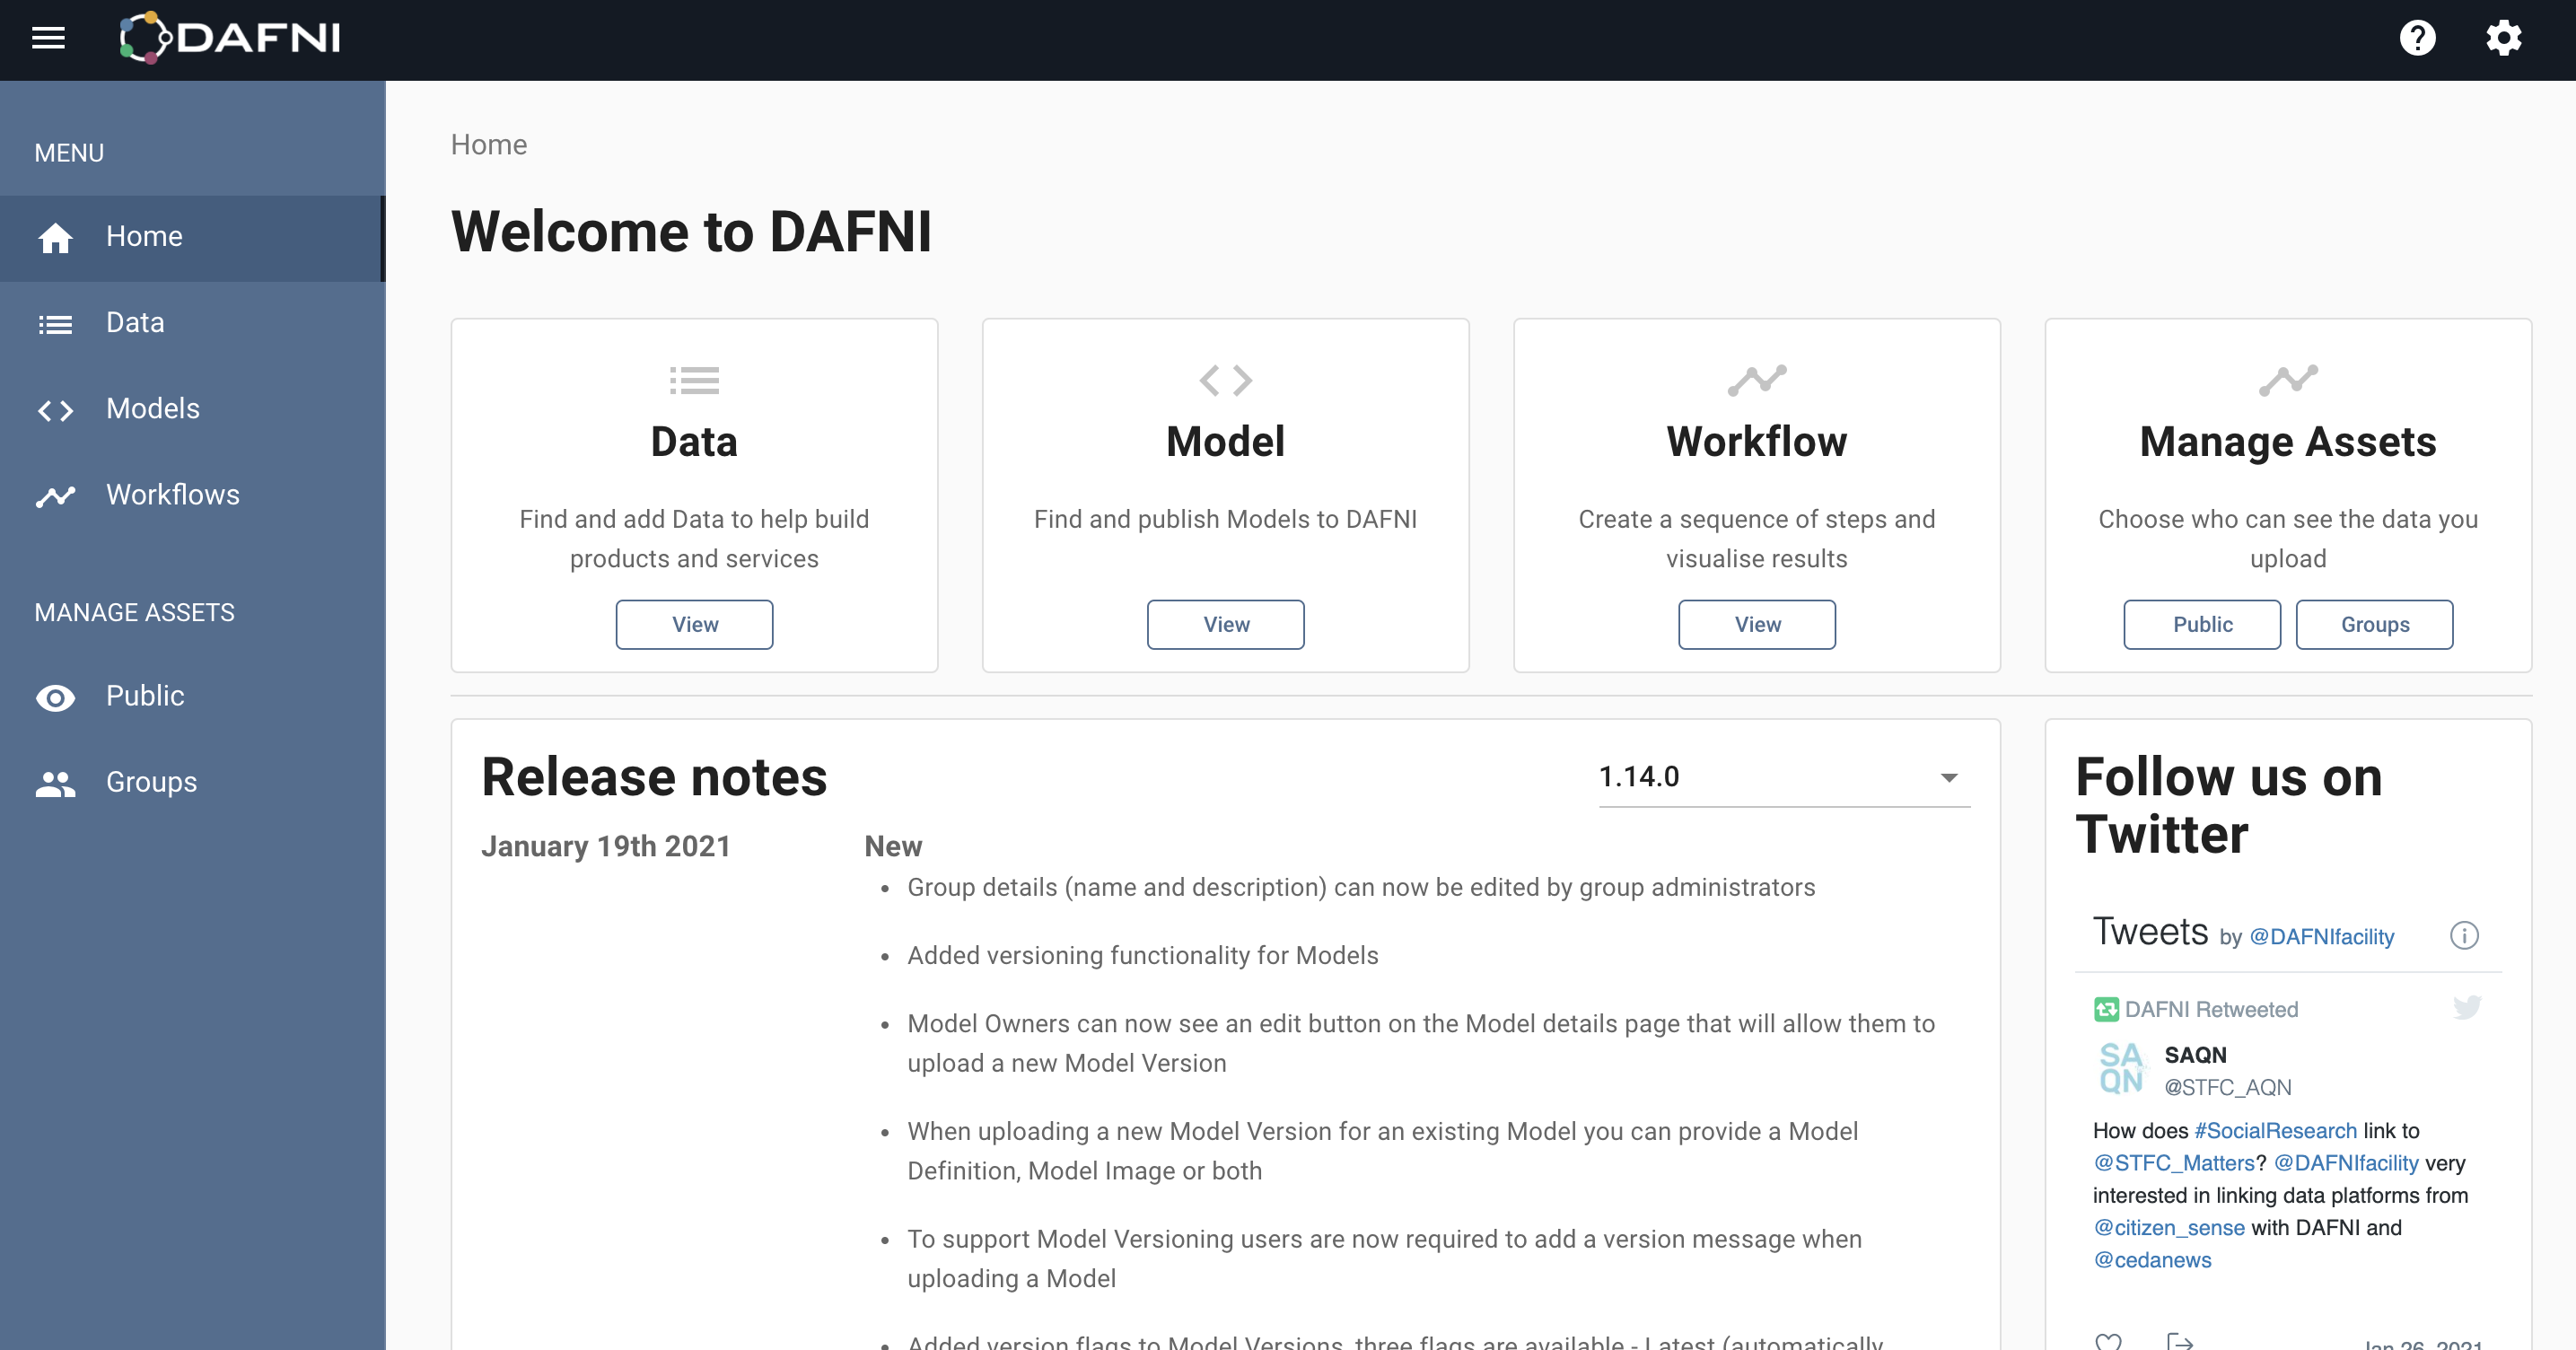
\includegraphics[width=0.8\linewidth]{figures/dafni-GUI.png}
\end{center}


}

\sframe{DAFNI workflow for coupled model}{

\centering

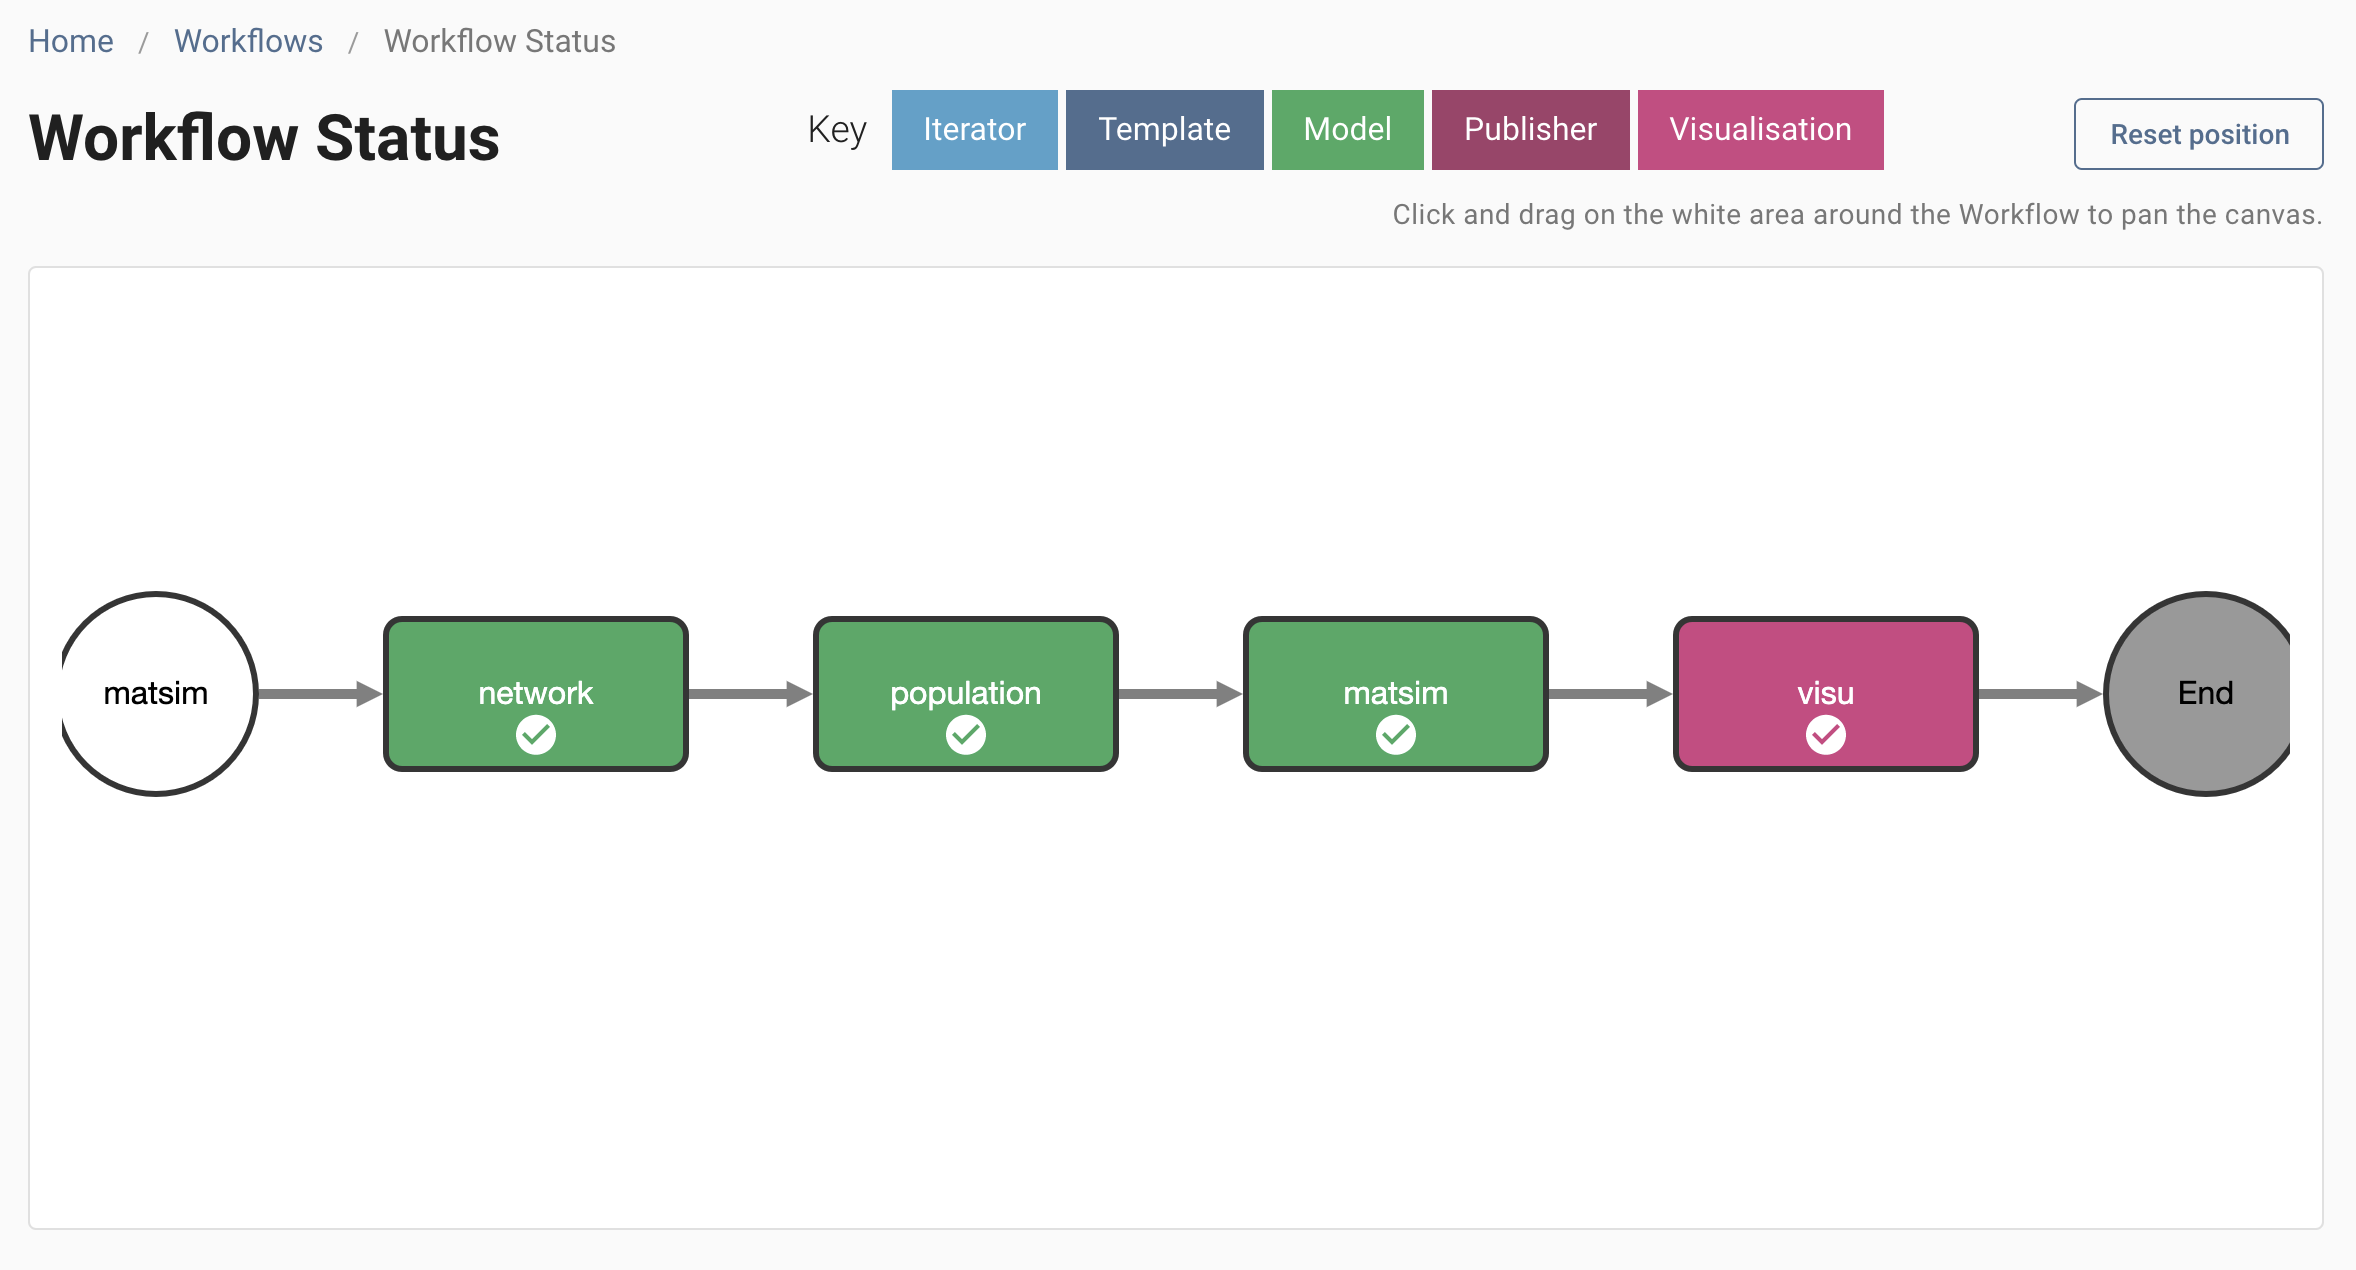
\includegraphics[width=\linewidth]{figures/matsim_workflow.png}

%  Construction of the transport model using the DAFNI workflow system: DAFNI workflow including model steps and a computational experiment (Monte Carlo simulations)

}

\sframe{Monte Carlo experiments}{

\centering

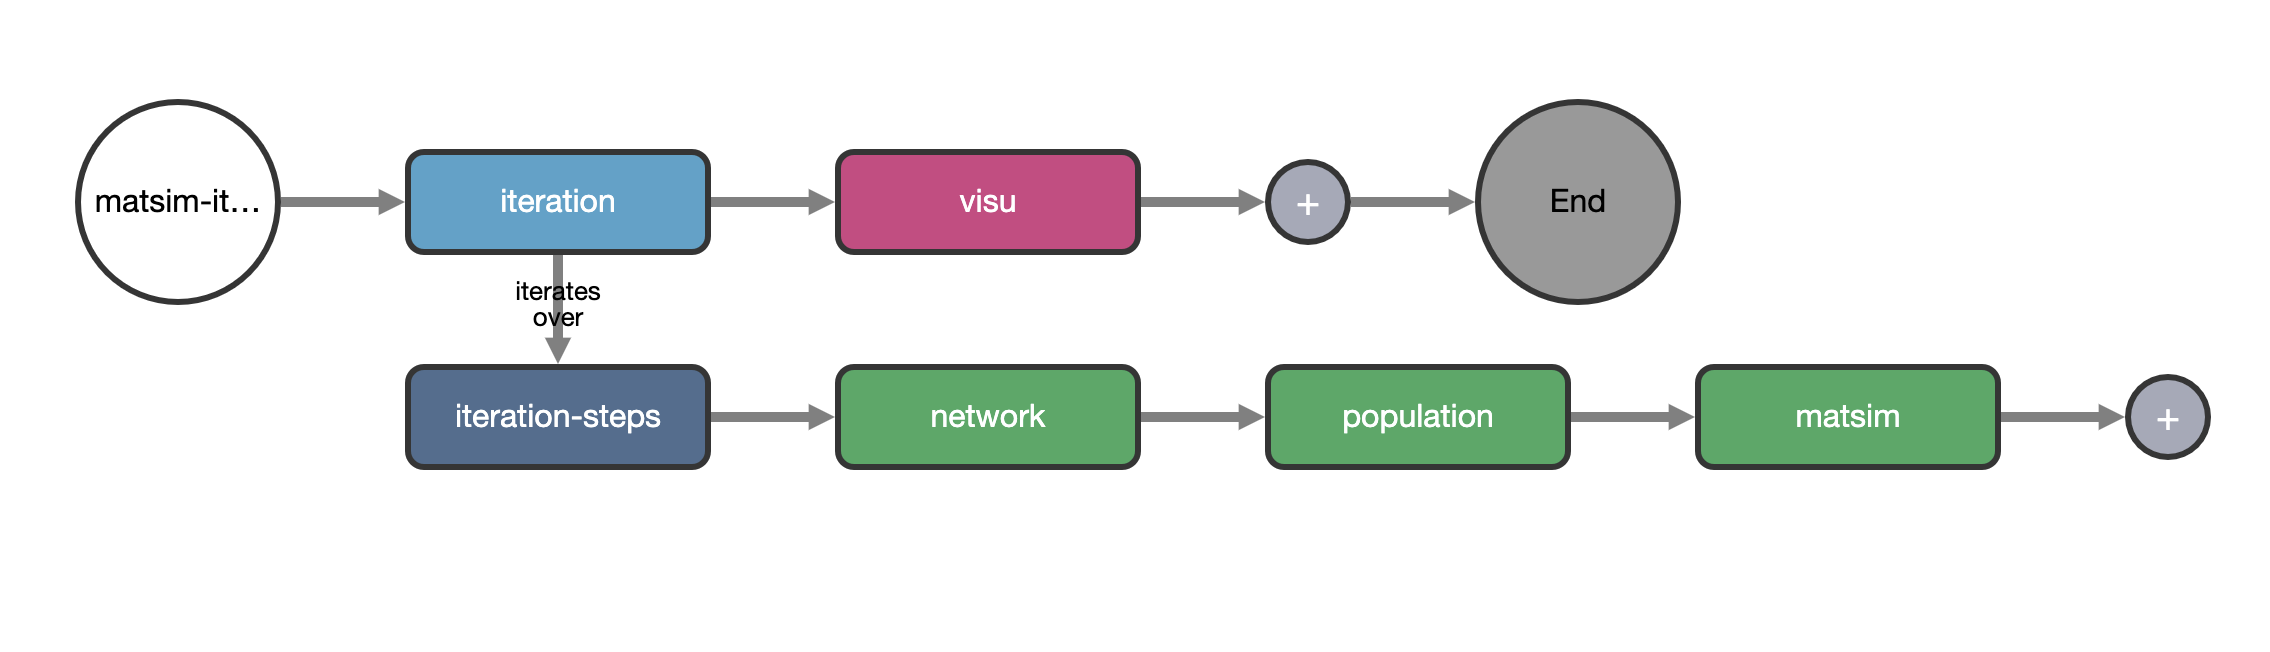
\includegraphics[width=\linewidth]{figures/matsim-iterations_workflow.png}

}

% The model is run on the largest functional urban areas (following the definition of (Florczyk et al., 2019)) in the UK. 

\sframe{Visualization within DAFNI}{

\begin{center}
	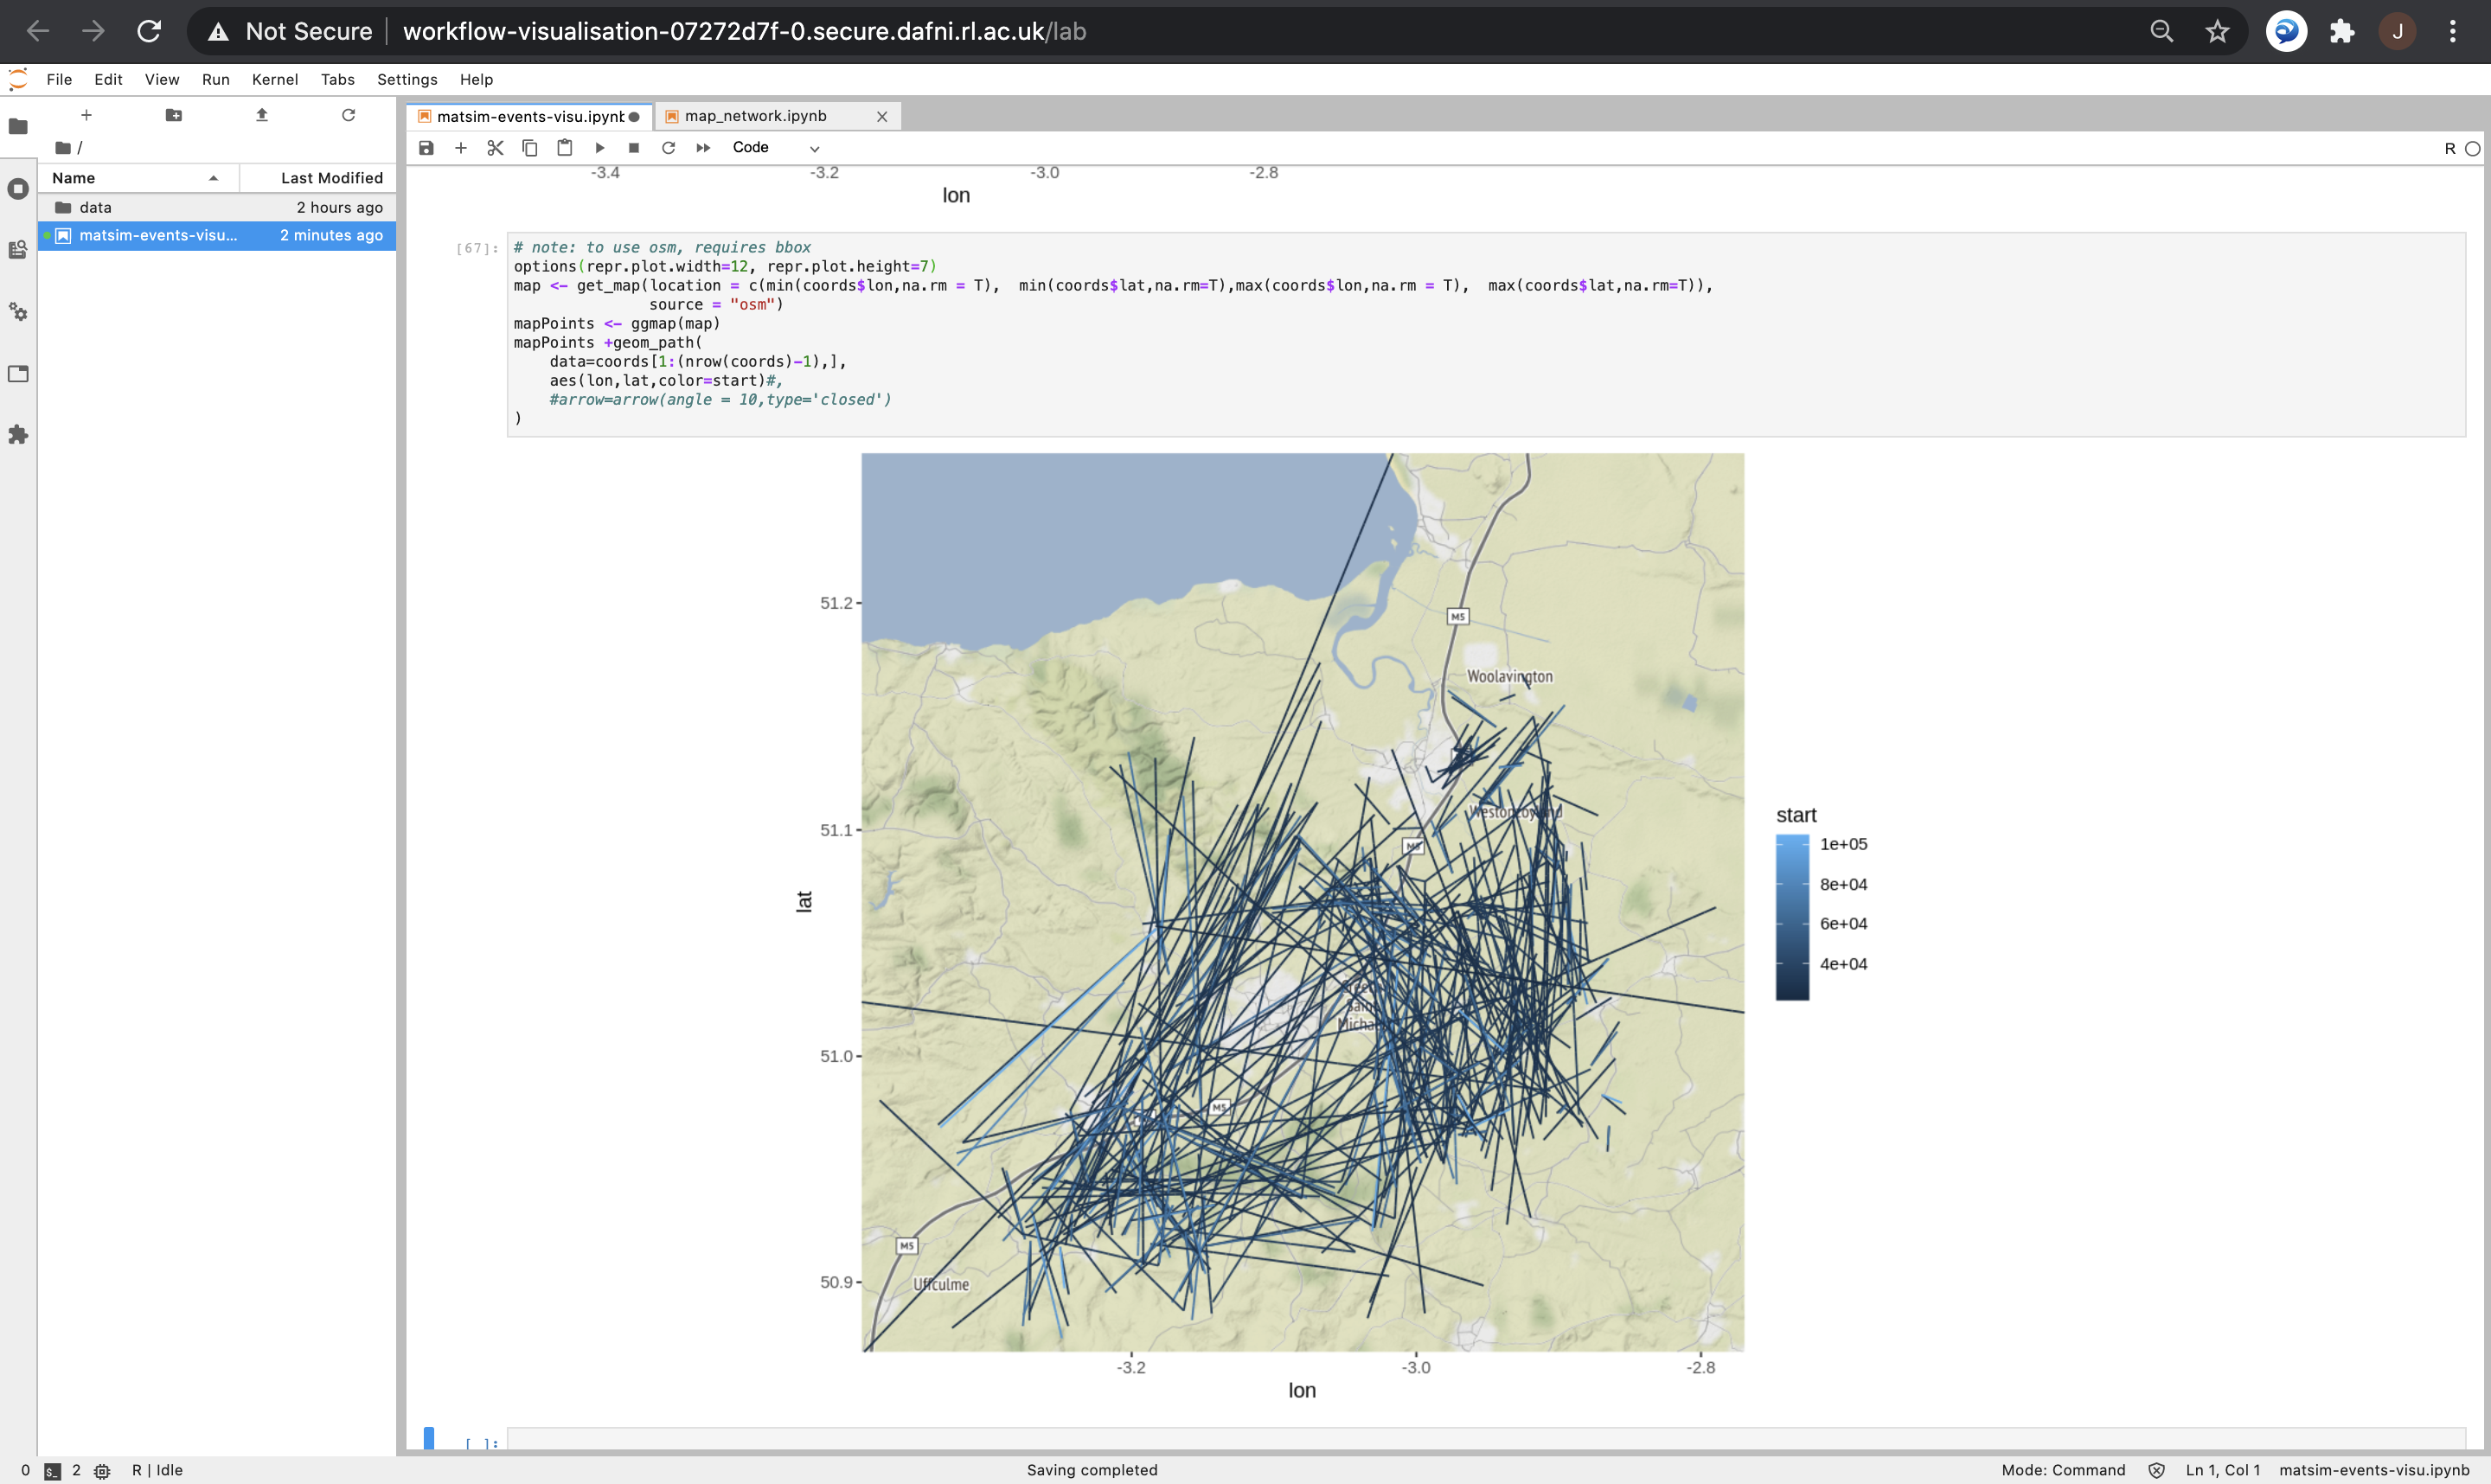
\includegraphics[width=\linewidth]{figures/visu_trips.png}	
\end{center}

}




\sframe{Simulation results: travel distances}{

% We show first results of numerical experiments studying the role of stochasticity on model outputs, for example in Figure 2 for the statistical distribution of trip departure times (these are iteratively evolved by agents in the MATSim model) for the urban area of Taunton. We also show in Figure 2 the distribution of car trip distances in the different urban areas, for 13 large urban areas (excluding London for performance purposes).

\begin{center}
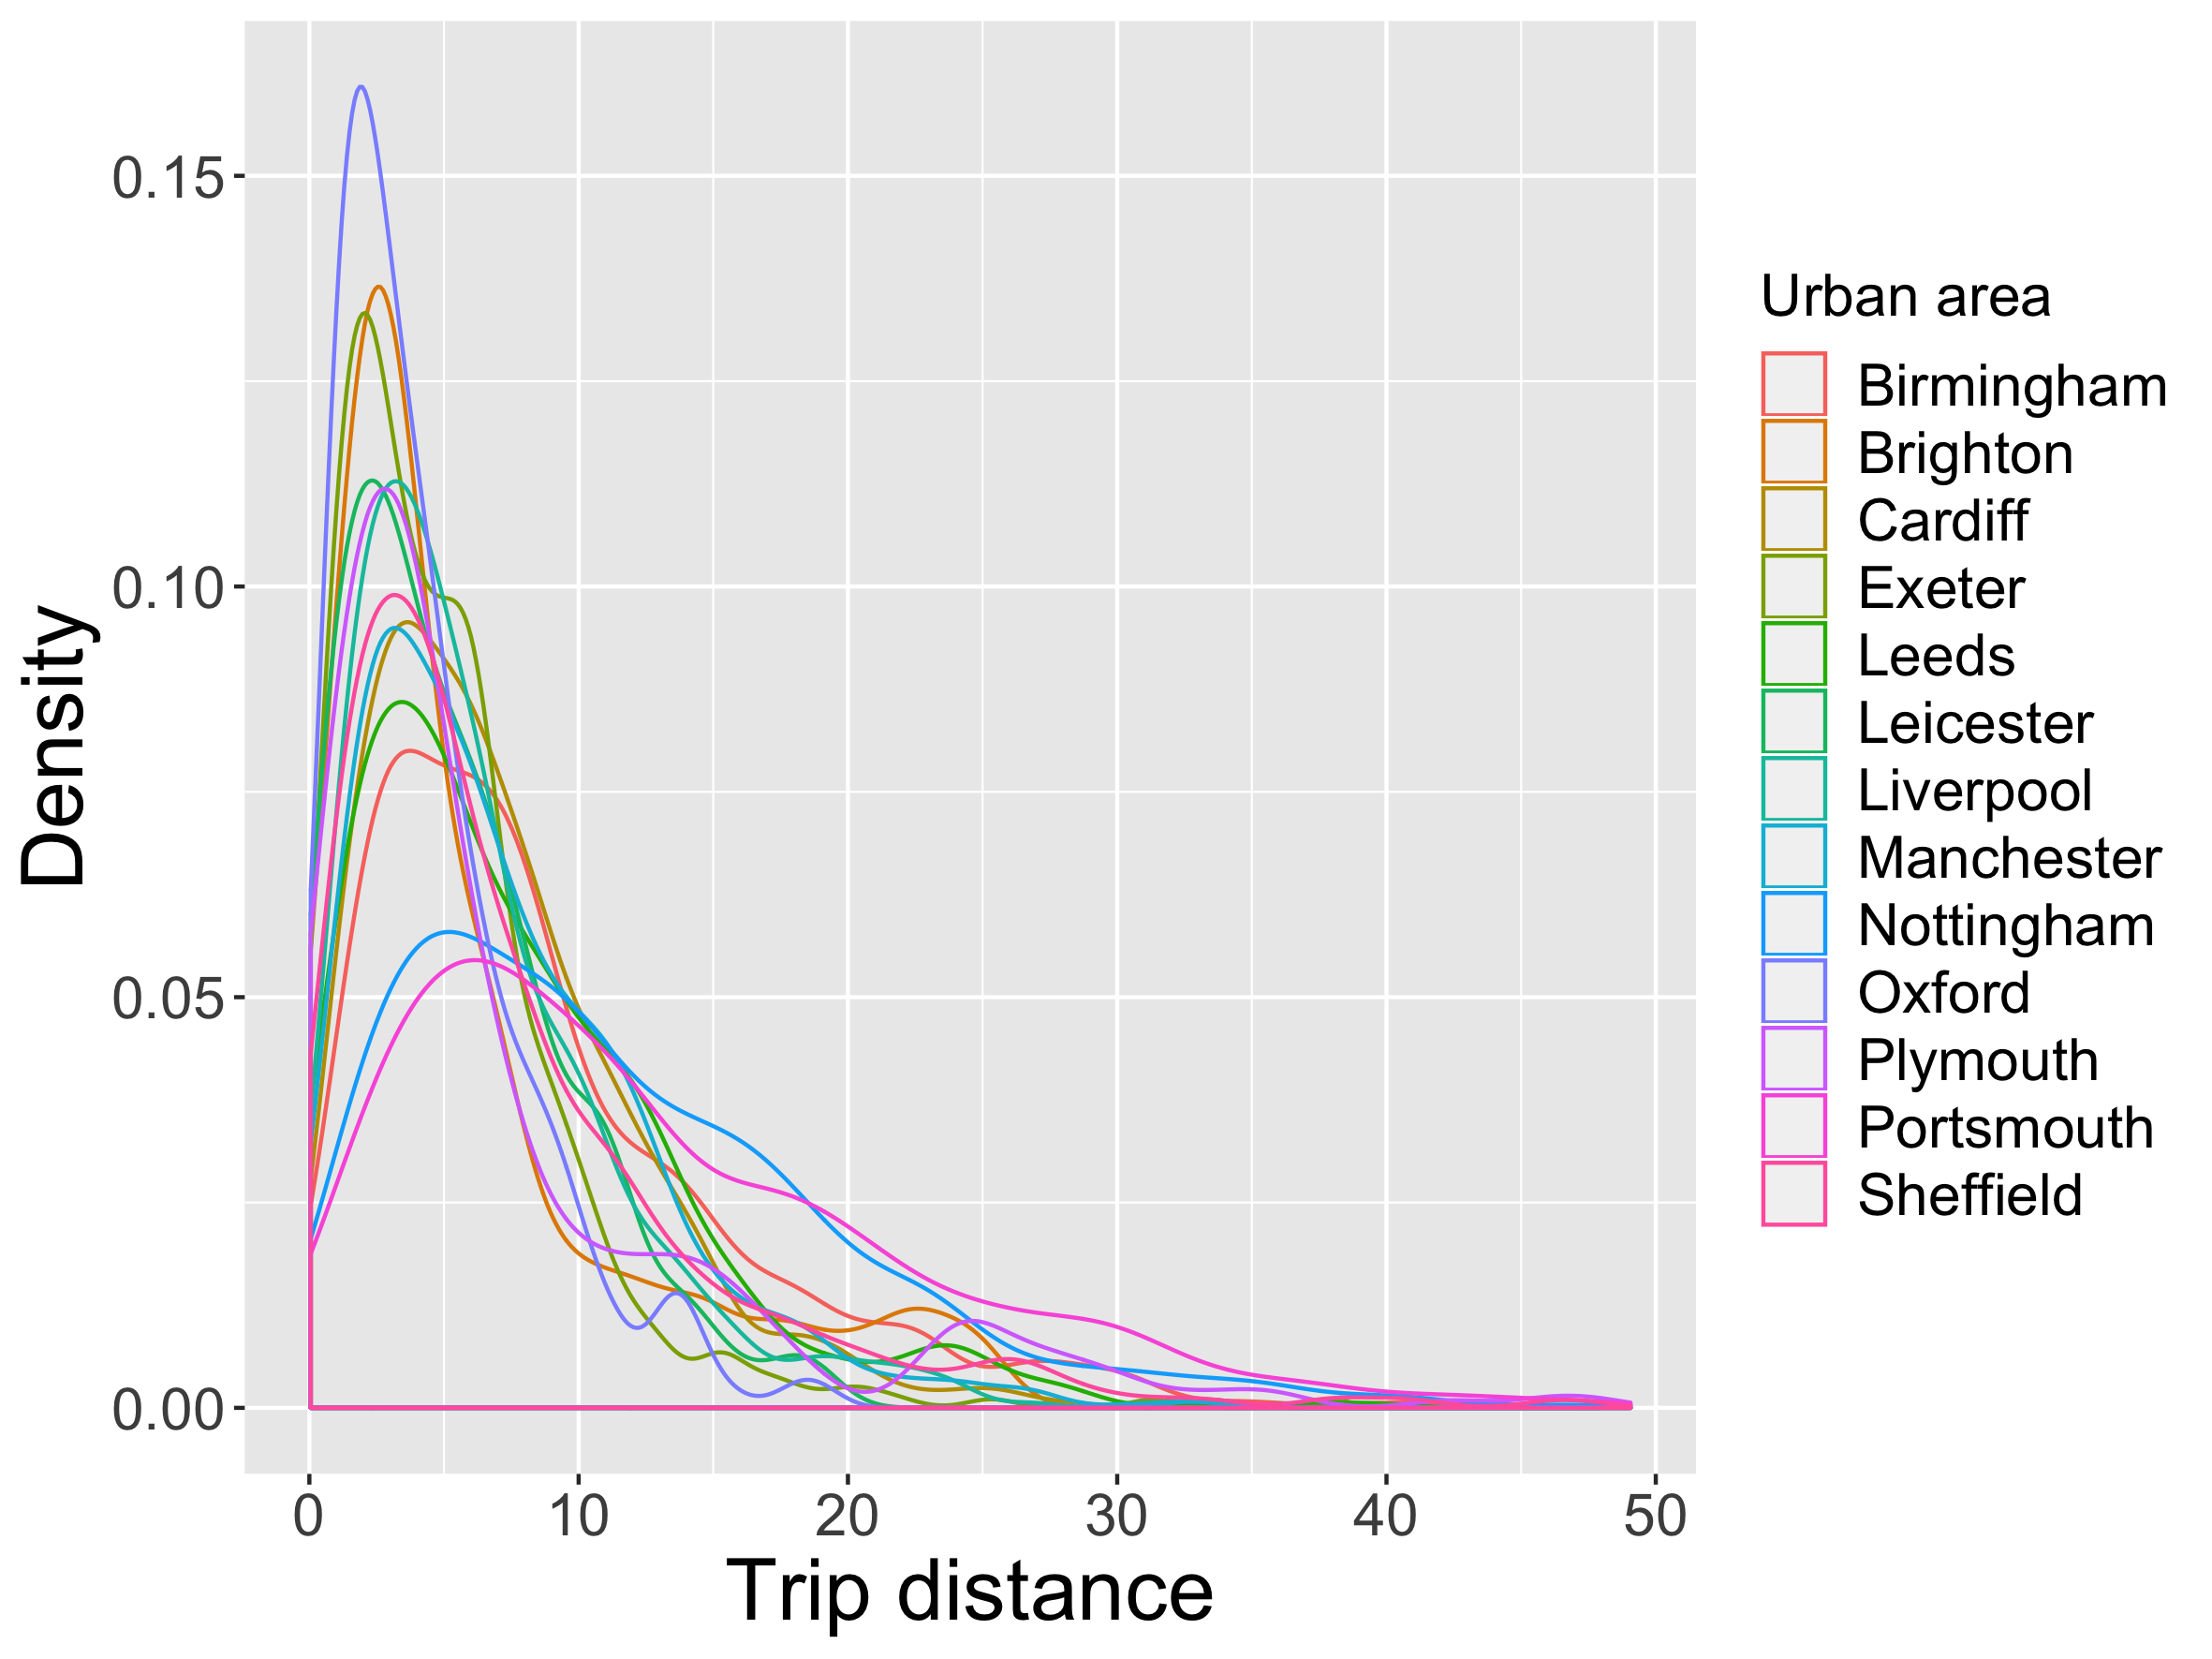
\includegraphics[width=0.9\linewidth]{figures/distances_allFUAs.png}
\end{center}

}

\sframe{Daily travel patterns}{

\begin{center}
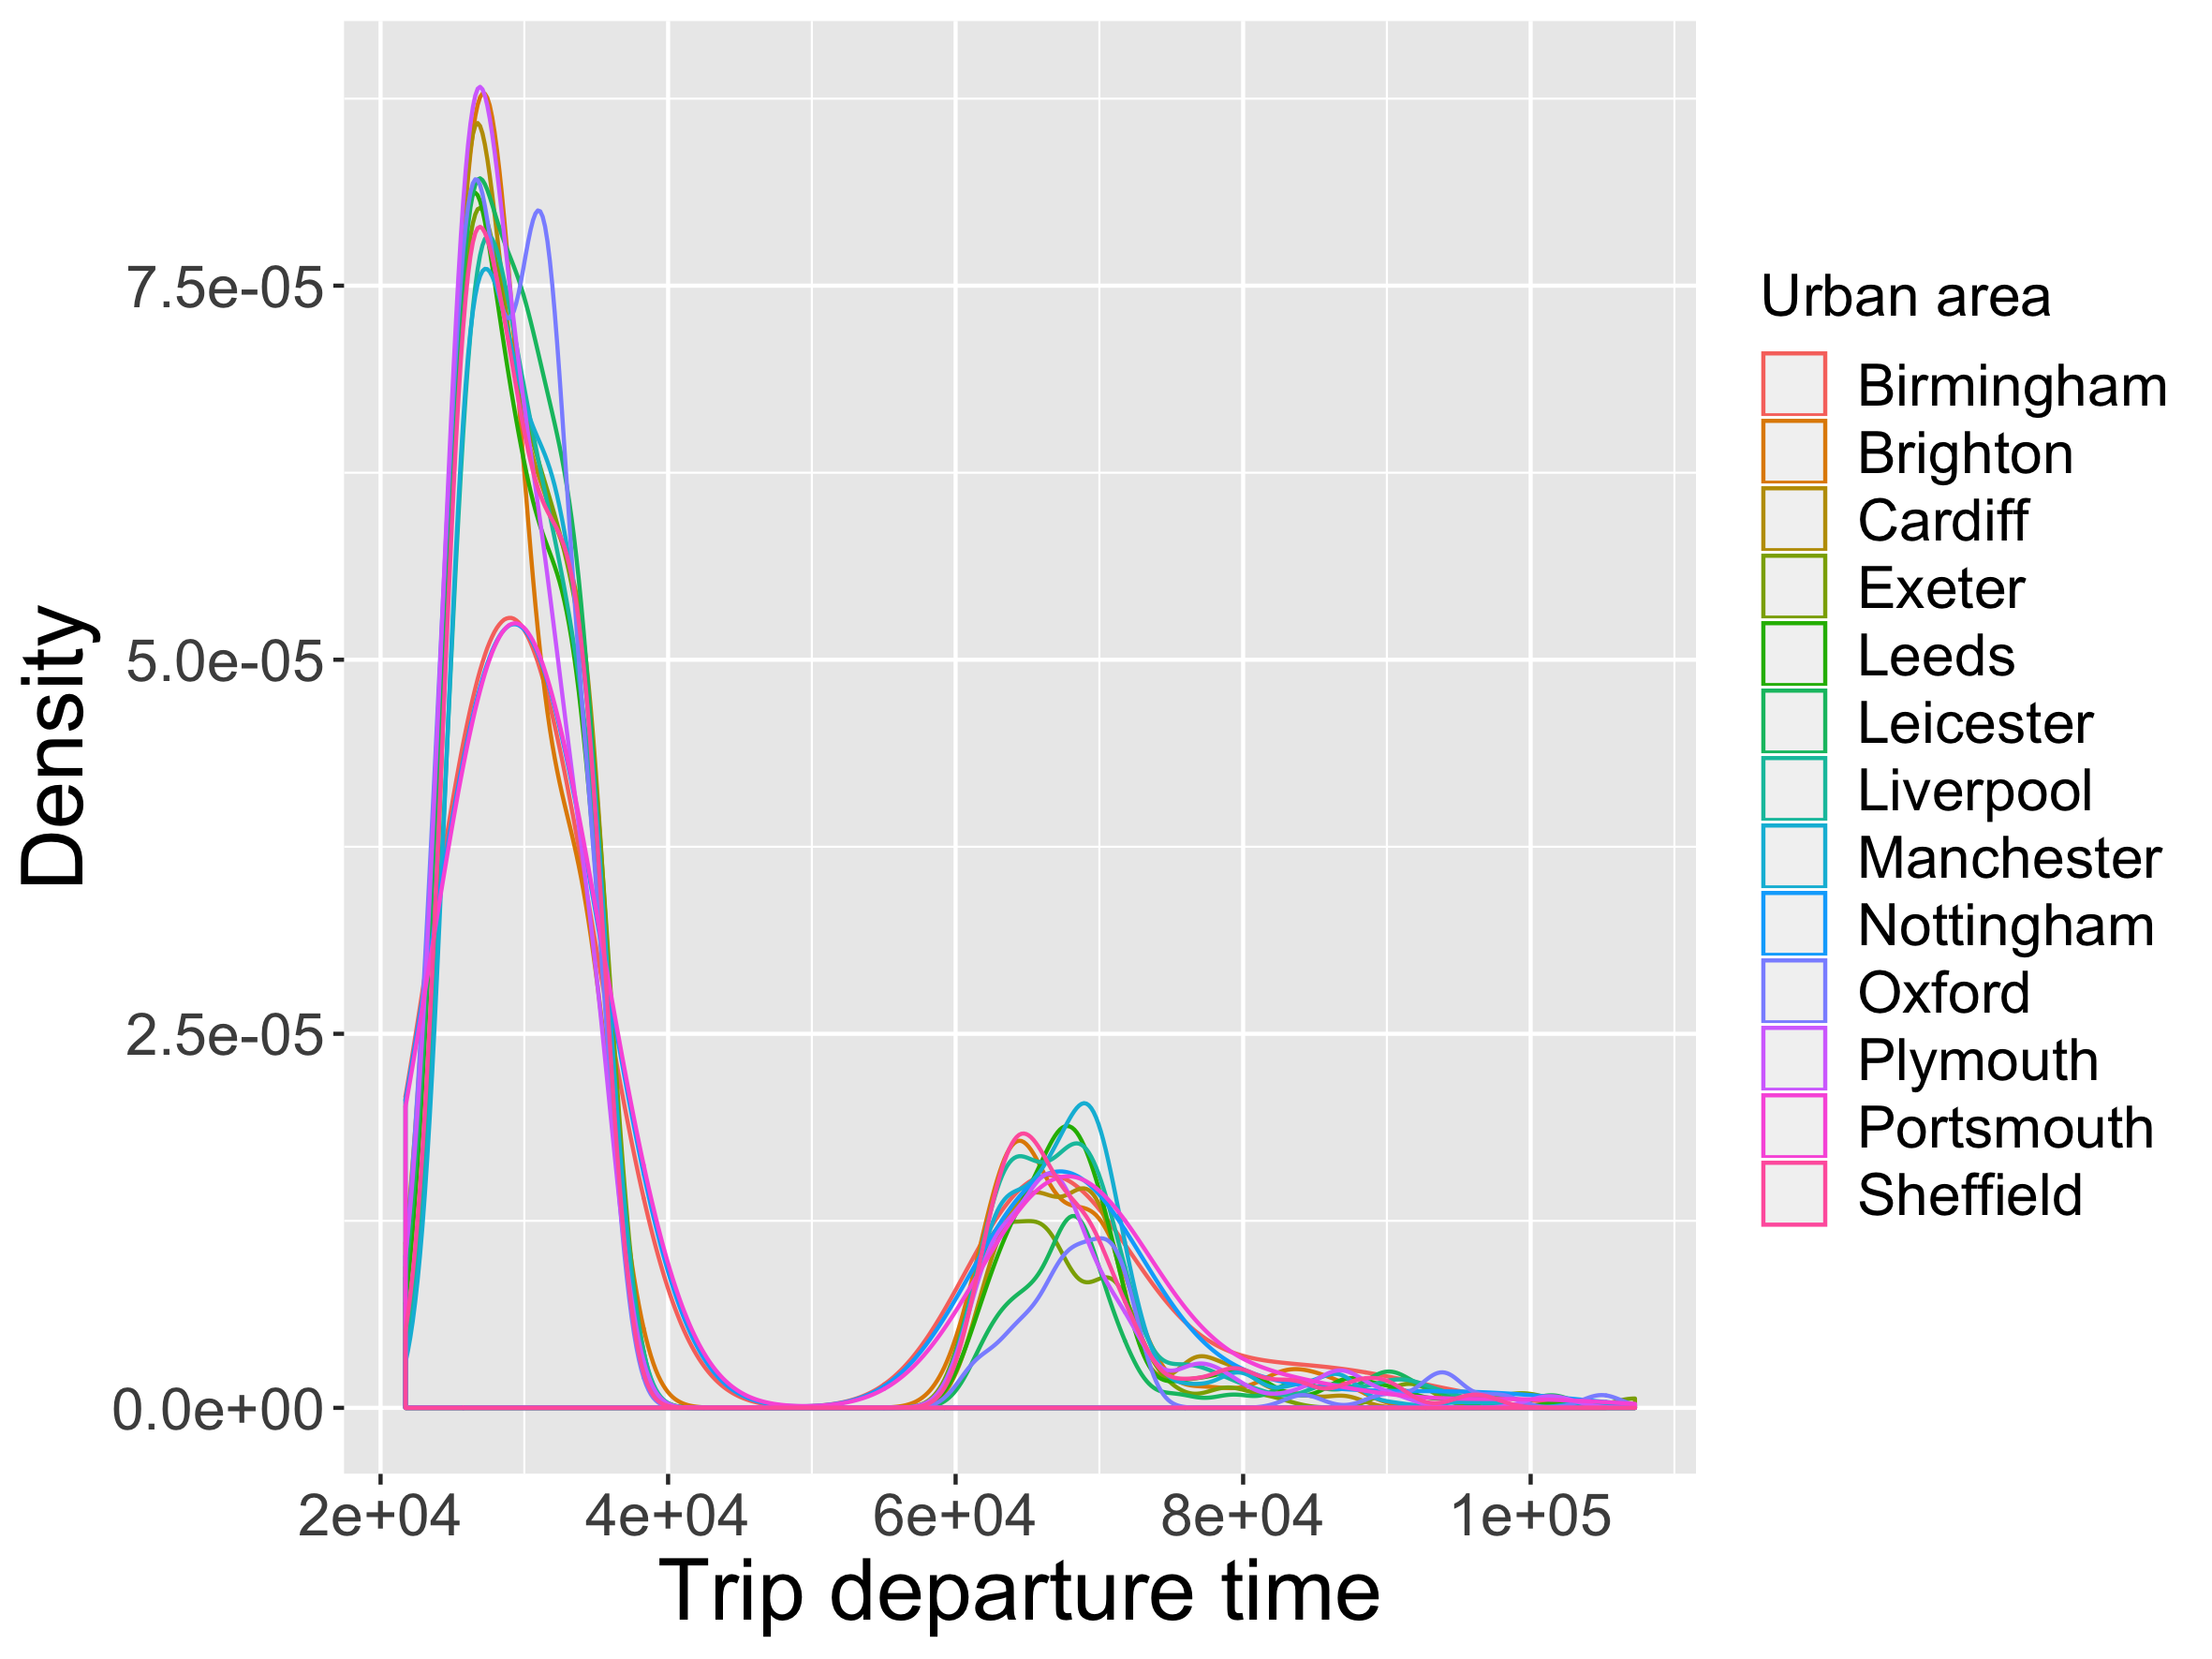
\includegraphics[width=0.9\linewidth]{figures/departuretimes_allFUAs.png}
\end{center}

% Results of the simulation of the integrated model on the largest functional urban areas in the UK. (Left) Distribution of trip departure times, for several stochastic repetitions on the same urban area; (Right) Distribution of trip distances for all urban areas (London was not included yet for performance reasons as numerical experiments are still being streamlined).

}



\sframe{Role of stochasticity}{

\begin{center}
	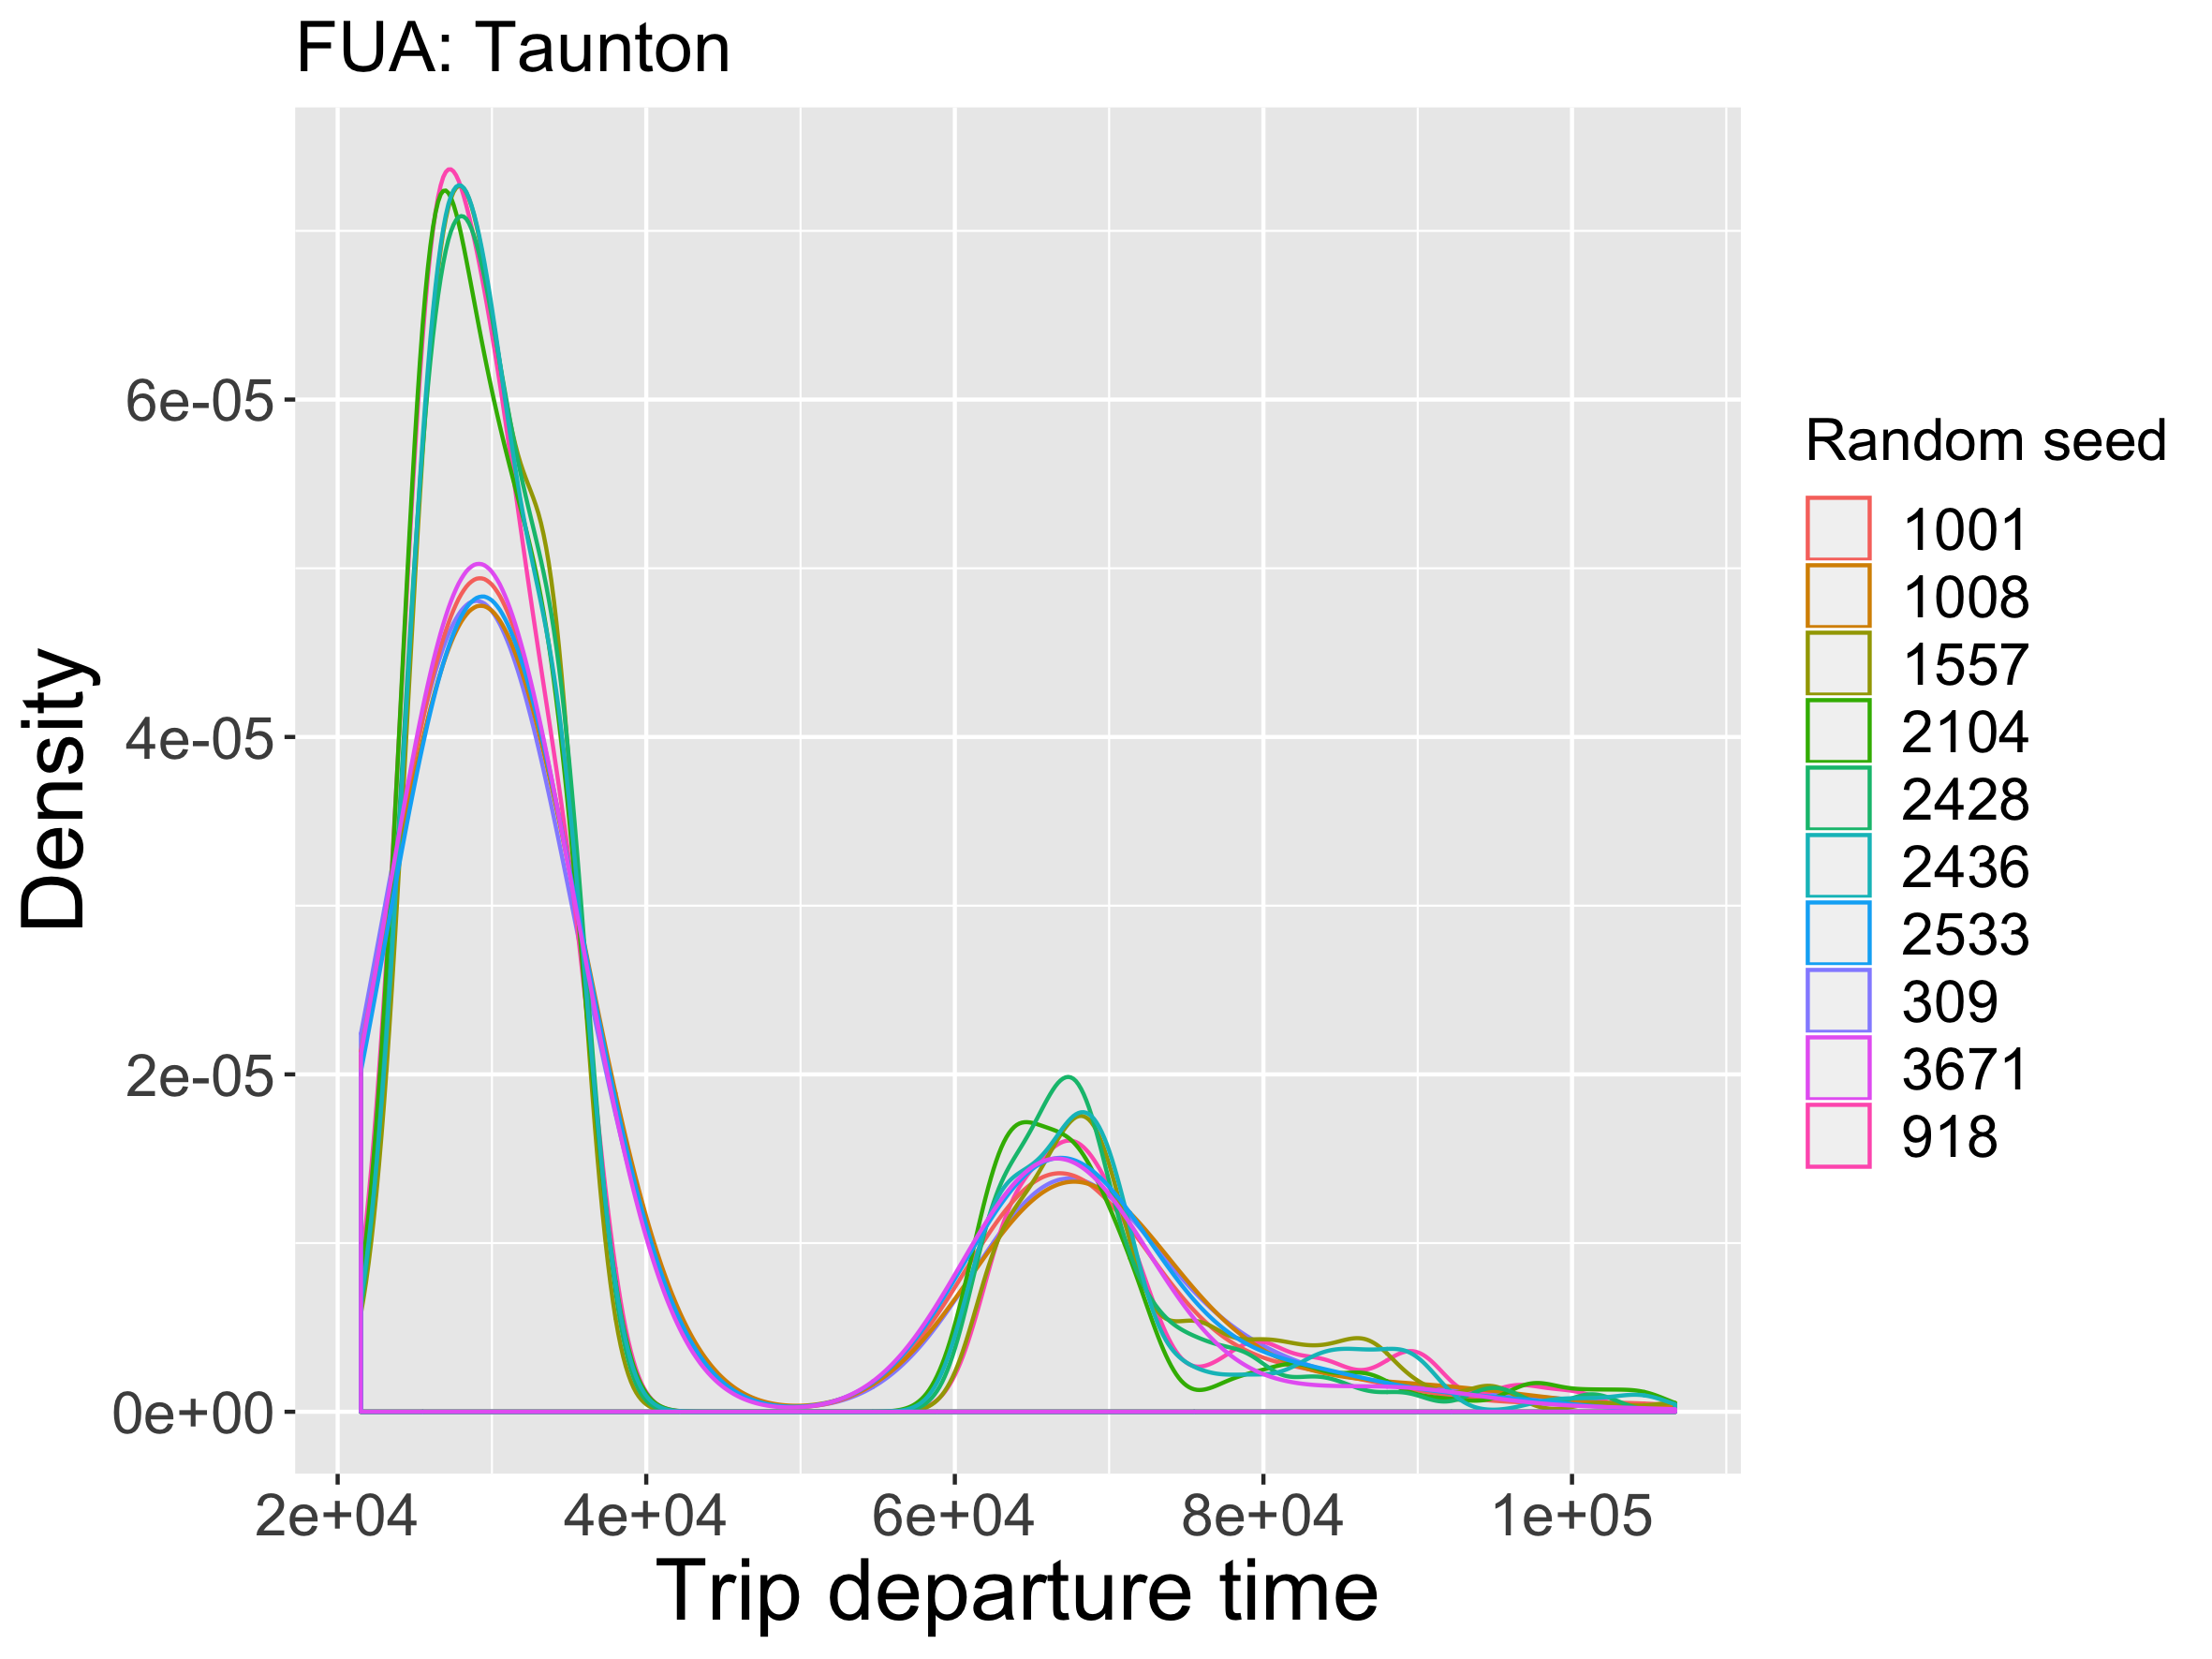
\includegraphics[width=0.9\linewidth]{figures/stochasticity_Taunton.png}	
\end{center}


}


\sframe{Validation: towards spatial sensitivity analysis}{


% For example, studying the role of spatial configuration on model outcomes (Raimbault et al., 2019) would be relevant to understand the influence of missing or imprecise data and sampling for the synthetic population. Furthermore, the implementation as open source OpenMOLE scripts embedding open models is an asset for an easier teaching of transport models, as these can seamlessly be run and explored by students without the need to access particular resources or proprietary software (Carrington & Kim, 2003).

\centering

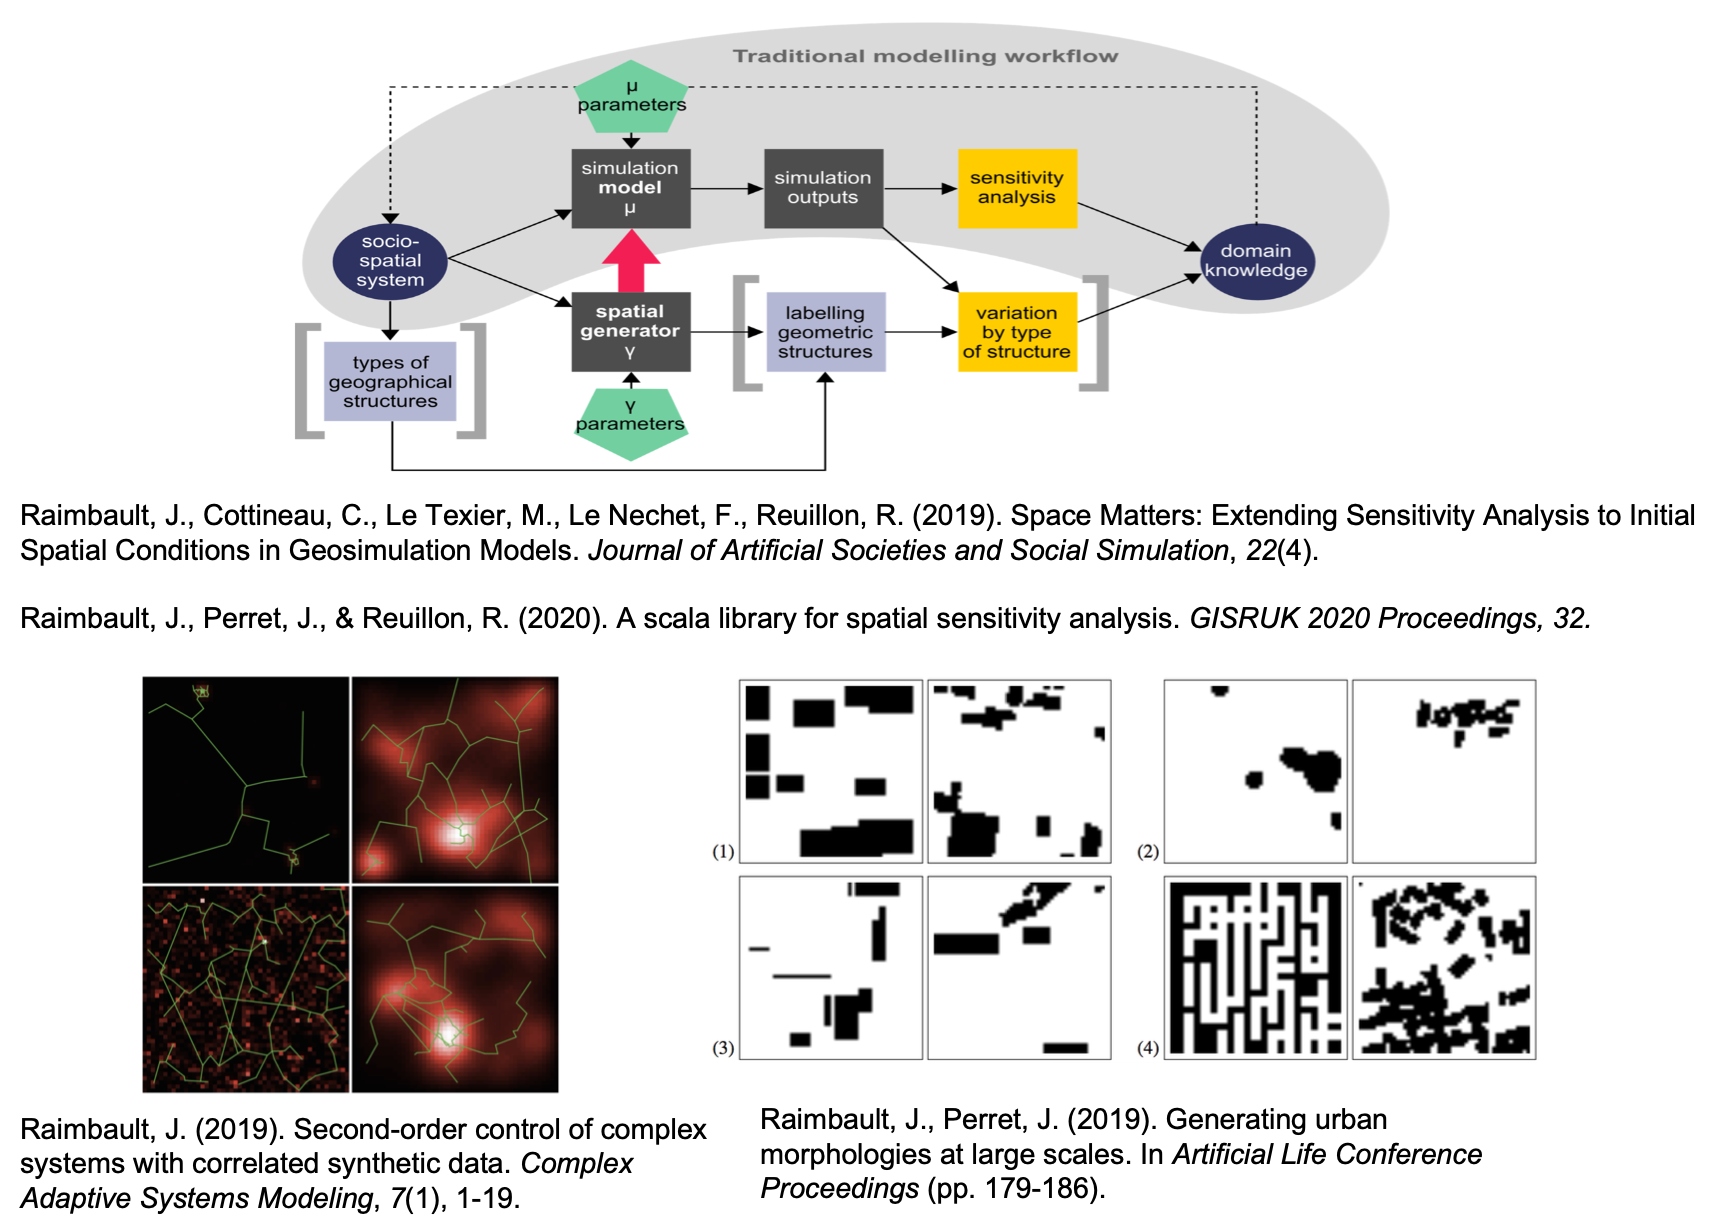
\includegraphics[width=0.95\linewidth]{figures/spatial_sa.png}

}





\section{OpenMOLE}

%Source code to prepare the model components, input data, and docker containers is available on an open-source git repository at https://github.com/JusteRaimbault/UrbanDynamics. To illustrate the reproducibility of our approach, we test the construction of the model with the OpenMOLE workflow engine (Reuillon, 2013), which provides a scripted workflow engine and methods to calibrate and validate simulation models, and suggest advanced numerical experiments for the validation of the coupled model. 

\sframe{OpenMOLE workflow engine}{



OpenMOLE model exploration open source software \cite{reuillon2013openmole}

\medskip

\begin{center}

\includegraphics[height=0.13\textheight]{figures/iconOM.png}

\includegraphics[height=0.13\textheight]{figures/openmole.png}
\end{center}

\medskip

\textit{Enables seamlessly (i) model embedding; (ii) access to HPC resources; (iii) exploration and optimization algorithms}

\medskip

\url{https://openmole.org/}

}

\sframe{Coupling SPENSER and QUANT with OpenMOLE}{

\centering

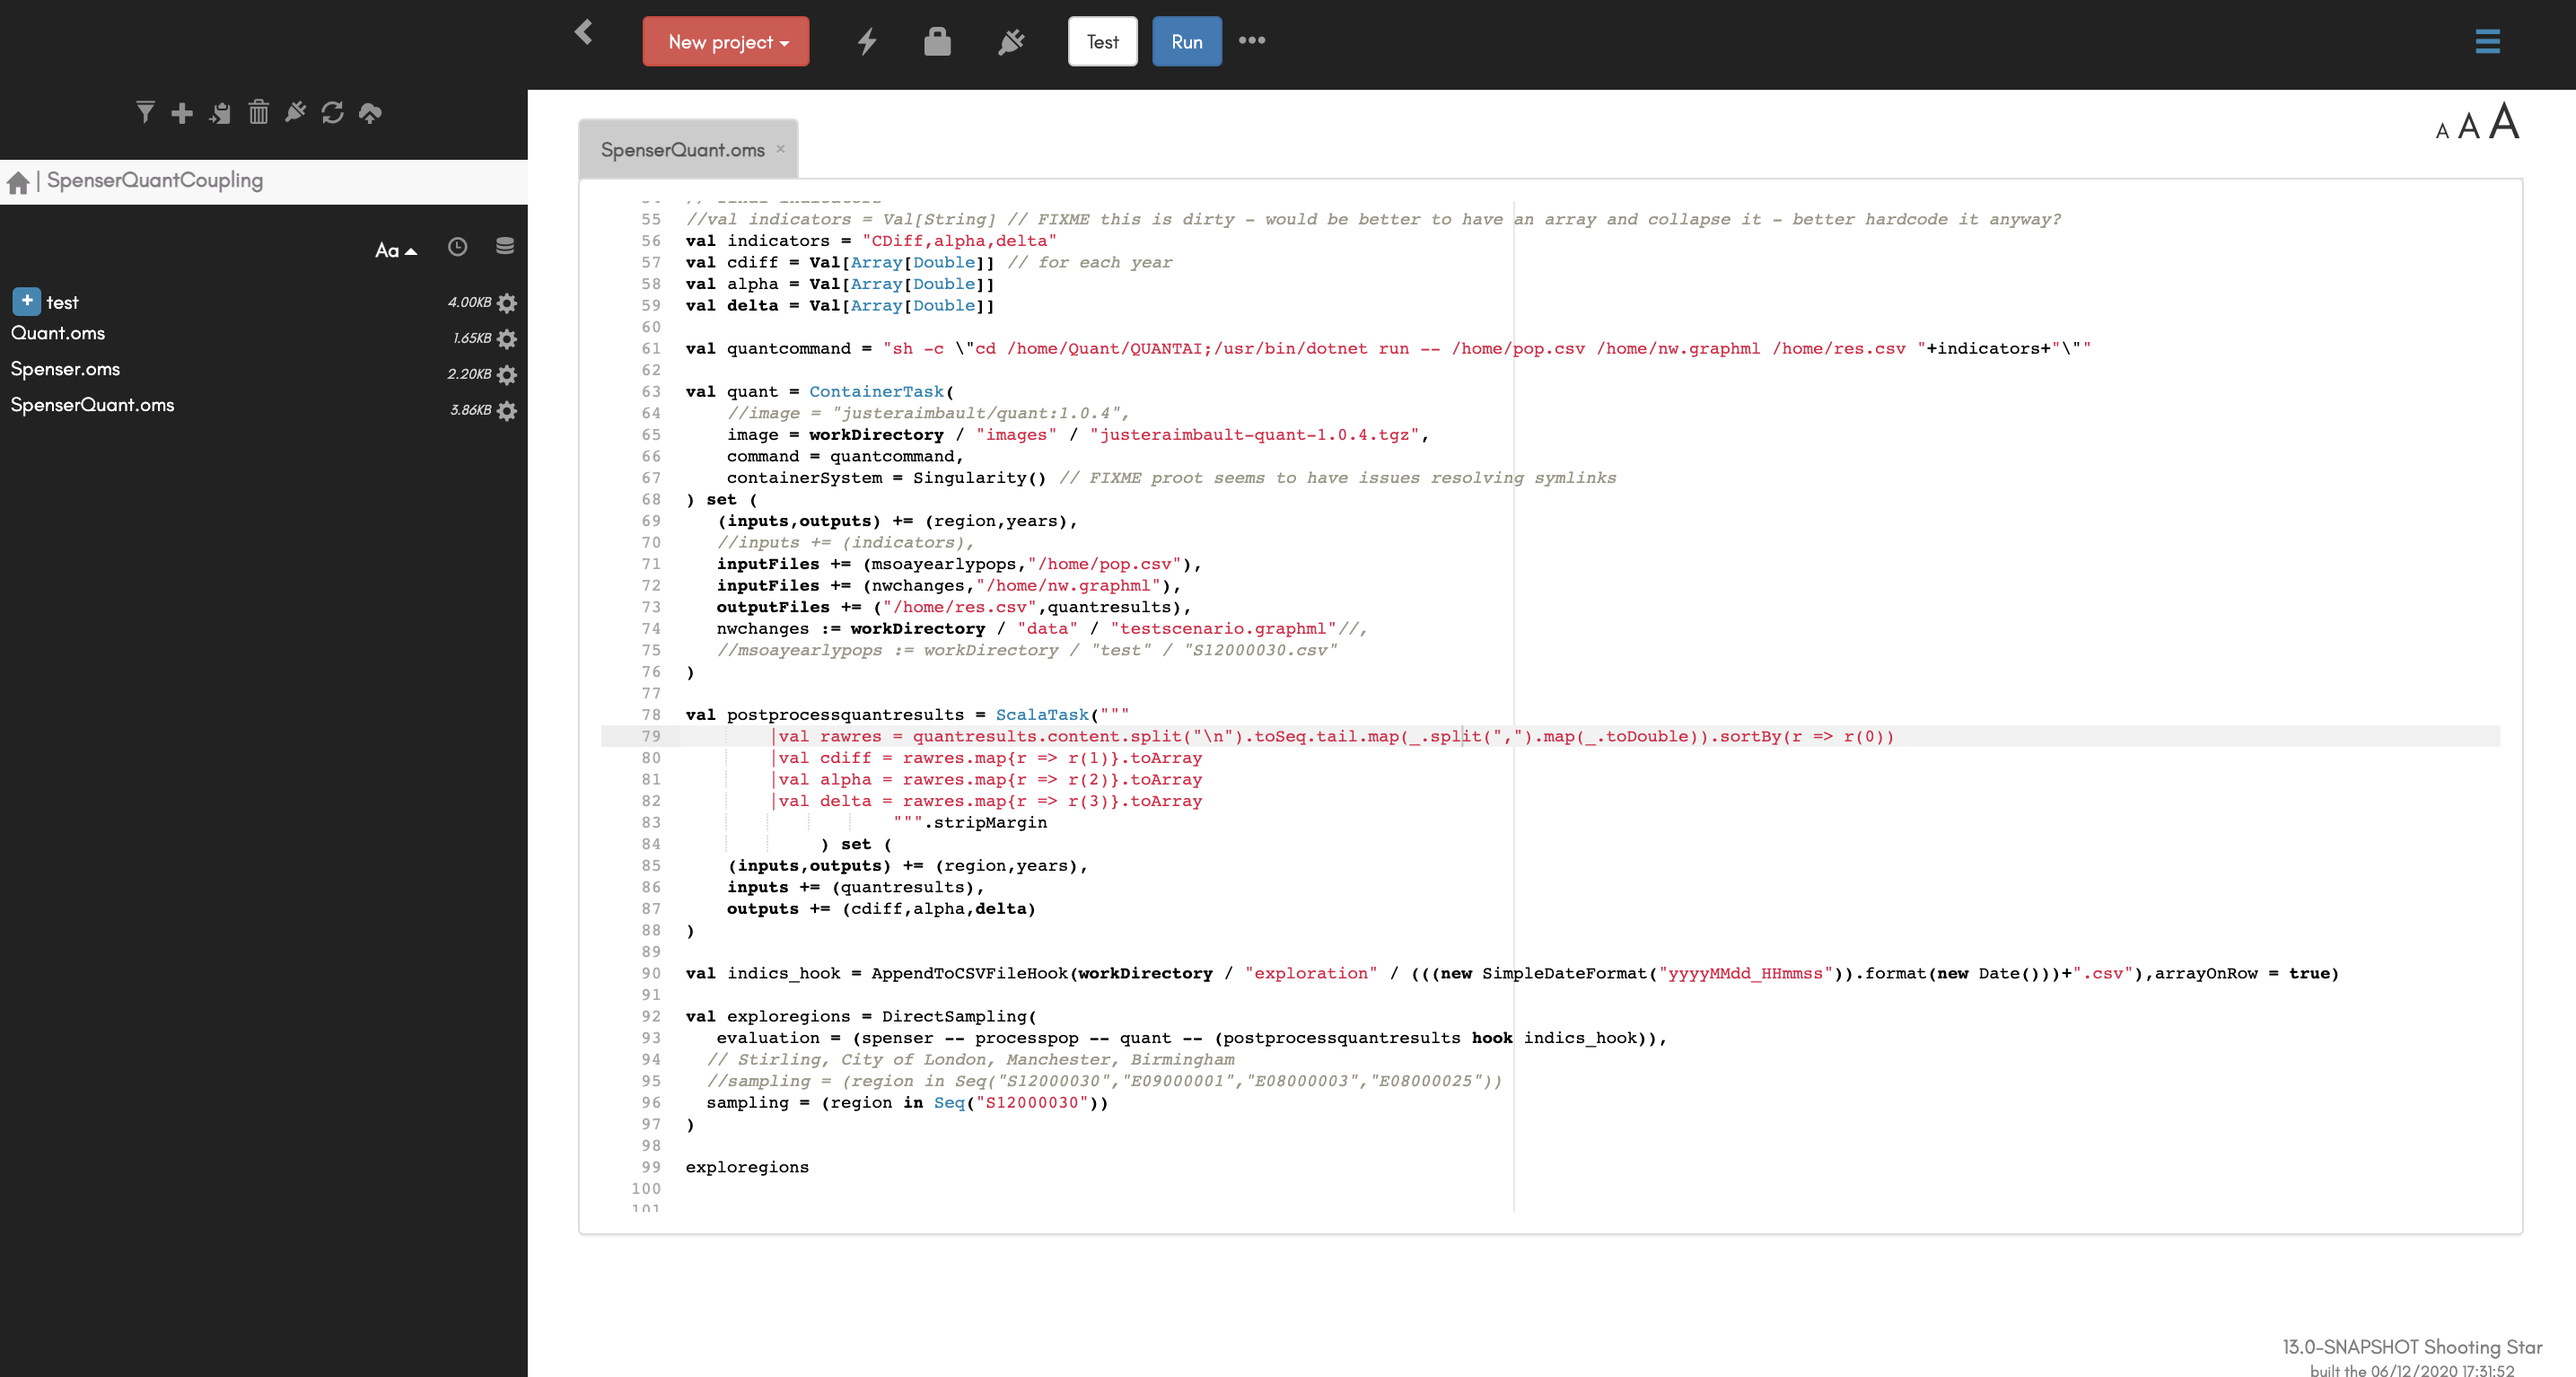
\includegraphics[width=\linewidth]{figures/openmole-spenserquant.png}

}

\sframe{Towards advanced validation experiments}{

\textbf{OpenMOLE integrates methods for: } sensitivity analysis, spatial sensitivity analysis, design of experiments, calibration, diversity search, inverse problems, model reduction.

\bigskip

\begin{center}
	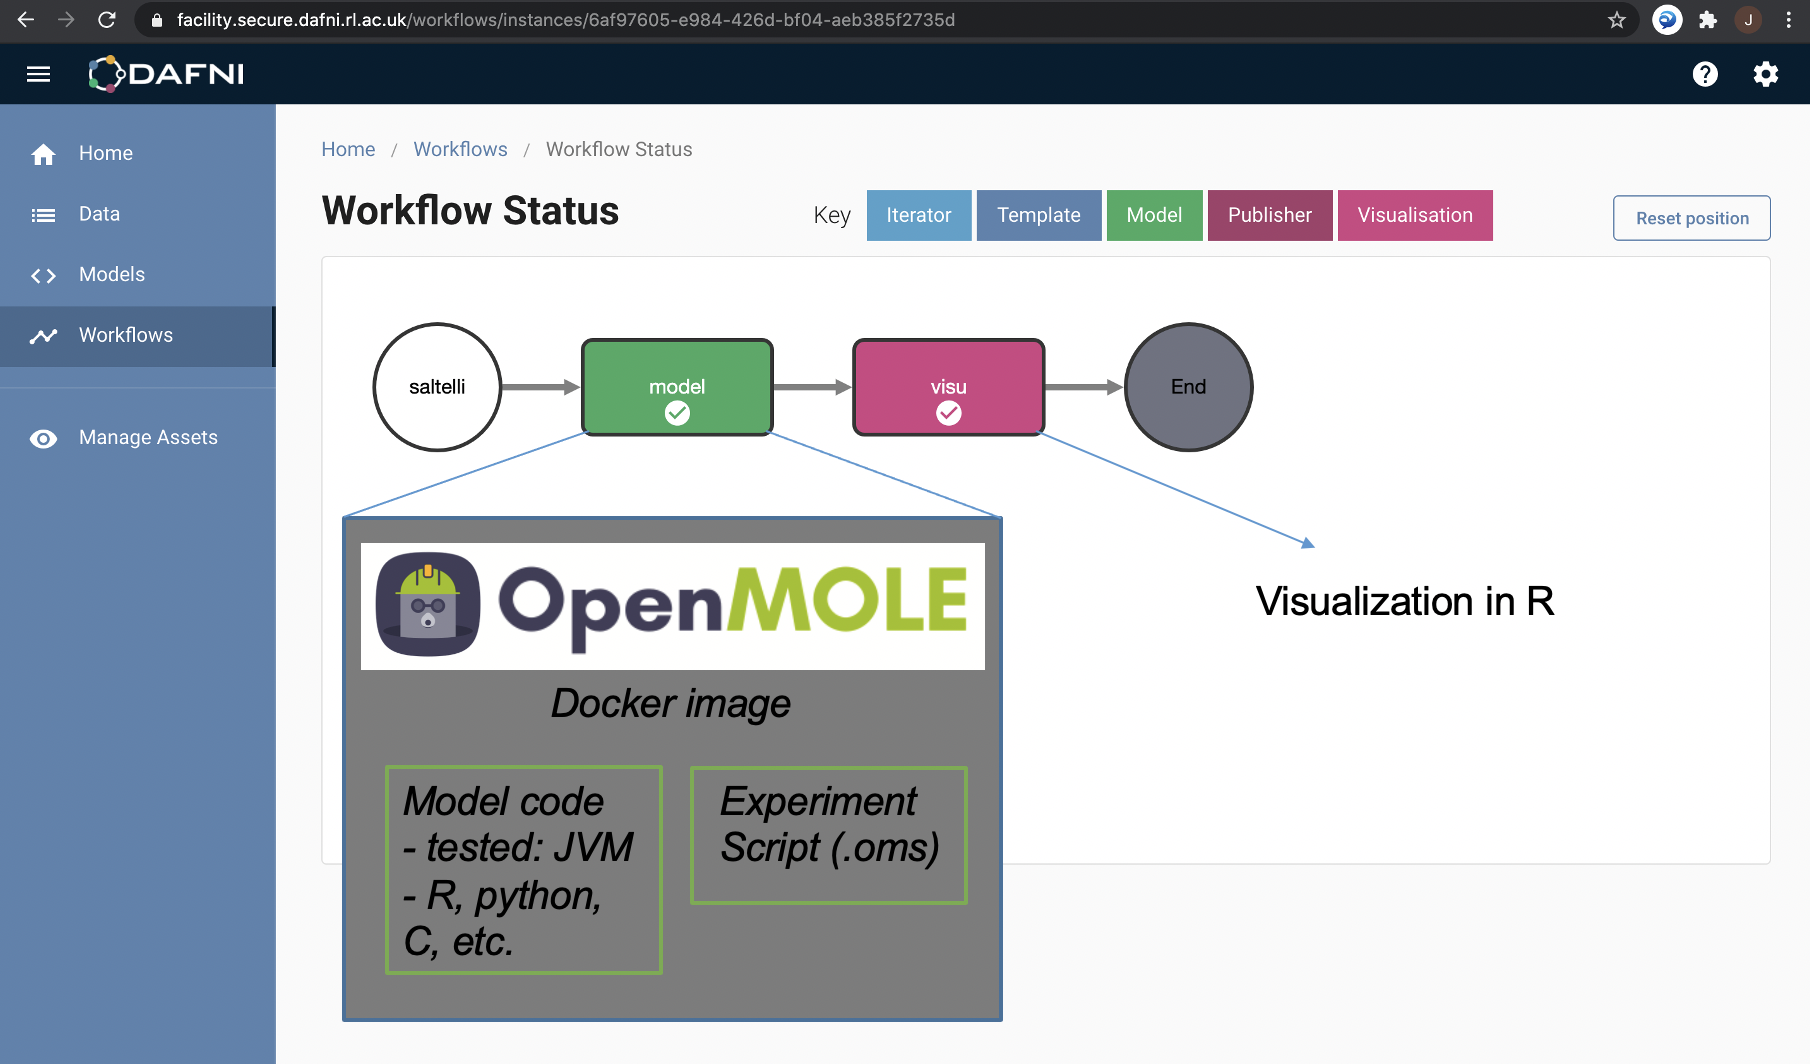
\includegraphics[width=0.75\linewidth]{figures/dafni-oml.png}
\end{center}

\textit{Integration of OpenMOLE into DAFNI}

}


\section{Discussion}

%Work in progress includes the application of this model to the development of health indicators within public transportation, and more particularly linking transportation and work-from-home policies with effective densities in public transport which provide potential exposure indicators in the context of the COVID-19 crisis. While urban density in itself is not significantly linked to stronger transmission (Hamidi et al., 2020), possible transmission within closed environment of public transport causes some concerns. The MATSim transport model has already been applied in the pandemic context: for example, Müller et al. (2020) build on the MATSim model to construct a full epidemiological agent- based model for the propagation of COVID-19 for the Berlin urban area. We limit our work to estimating public transport congestion and density, providing a measure of potential contacts between individuals. Our approach is therefore easier to test and validate, as less sub-models and aspects have to be tested, and we expect it to provide more robust conclusions on public transport itself. As our transport model can be systematically applied to any urban area in UK, we also expect to be able to test and compare policies across different urban and epidemiological contexts.


\sframe{Discussion}{

\textbf{Developments}

\medskip

%$\rightarrow$ Integration of QUANT to generate commuting plans
% => WIP
%\medskip

%$\rightarrow$ Construction of multimodal network data for MATSim
%=> WIP
%\medskip

$\rightarrow$ Dynamical strong coupling of QUANT and SPENSER

\bigskip

\textbf{Applications}

\medskip

$\rightarrow$ Validation of sub-models and integrated models using advanced model validation methods

\medskip

$\rightarrow$ Use MATSim outputs to quantify effective densities in public transport: potential exposure indicators in the COVID-19 context

\medskip

$\rightarrow$ Impact of policies and interventions on transport system dynamics and potential contaminations


}

\sframe{Health indicators for public transport}{

}



\sframe{Conclusion}{


$\rightarrow$ Open, reproducible and validated urban models as elementary bricks towards larger integrated models


\bigskip
\bigskip

\textbf{Open repositories}

\medskip

\url{https://github.com/JusteRaimbault/UrbanDynamics} for workflows

\medskip

\url{https://github.com/openmole/spatialdata} for data processing



\bigskip

\textbf{Workflow engines}

\medskip

DAFNI: \url{https://dafni.ac.uk/}

\medskip

OpenMOLE: \url{https://openmole.org}

The authors acknowledge the DAFNI platform for funding through the Champions program, and the funding of Urban Dynamics Lab Grant EPSRC EP/M023583/1.

}



%%%%%%%%%%%%%%%%%%%%%
\begin{frame}[allowframebreaks]
\frametitle{References}
\bibliographystyle{apalike}
\bibliography{biblio}
\end{frame}
%%%%%%%%%%%%%%%%%%%%%%%%%%%%




\end{document}

